\documentclass[../notes.tex]{subfiles}

\pagestyle{main}
\renewcommand{\chaptermark}[1]{\markboth{\chaptername\ \thechapter\ (#1)}{}}
\setcounter{chapter}{5}

\begin{document}




\chapter{Complex MO Diagrams}
\section{MO Theory: LCAOs and Group Orbitals}
\begin{itemize}
    \item \marginnote{10/31:}Last time: Building MO diagrams by qualitatively identifying a basis of atomic orbitals (e.g., 1s for H, 2s and 2p for F) and intuitively determining an axis to about which they transform within the linear point group $C_{\infty v}$.
    \item Today: Making this process more formal, as is necessary for more complex, polyatomic molecules.
    \item For polyatomic molecules, we need to determine how the basis atomic orbitals transform. This will allow us to approximate molecular orbitals with linear combinations of them (the AOs) that transform with the same symmetry.
    \begin{itemize}
        \item To do this, we need to understand how to group together valence atomic orbitals, i.e., how to construct \textbf{group orbitals}.
    \end{itemize}
    \item \textbf{Group orbital}: An MO of a complex molecule.
    \item Strategy for building group orbitals and creating the relevant MO diagram.
    \begin{enumerate}
        \item Determine the point group of the molecule. If it is a linear molecule, substituting a simpler point group that still retains the symmetry of the orbitals (ignoring the signs) makes the process easier by eliminating infinite-fold rotation axes.
        \begin{itemize}
            \item We will substitute the 2-fold \textbf{subgroup} of the relevant point group in these cases.
            \item In particular, substitute $D_{2h}$ for $D_{\infty h}$ and $C_{2v}$ for $C_{\infty v}$.
        \end{itemize}
        \item Assign $xyz$ coordinates.
        \item Construct reducible representations for the valence orbitals on the peripheral atoms.
        \item Reduce each representation to its IRRs (i.e., find the symmetry of the group orbitals). Group orbitals are the combinations of atomic orbitals that match the symmetry of the IRRs.
        \item Identify the atomic orbitals on the central atom with the same symmetries (IRRs) as those found in step 4.
        \item Combine the atomic orbitals with matching symmetry and similar energy. The total number of MOs must be equal to the number of atomic orbitals used from all the atoms.
        \begin{itemize}
            \item Energy scaling of MOs $\sigma<\pi<\text{lone pairs}<\pi^*<\sigma^*$. More nodes equals higher in energy.
        \end{itemize}
        \item Label MOs.
        \begin{itemize}
            \item $\sigma$ implies a SALC with infinite-fold rotational symmetry about the bond axis; $\pi$ implies a SALC with 2-fold rotational symmetry about the bond axis.
            \item No superscript implies a bonding interaction; superscript $*$ implies an antibonding interaction.
            \item Subscript $g$ implies symmetrical with respect to inversion; subscript $u$ implies asymmetrical with respect to inversion.
        \end{itemize}
        \item Fill in the electrons.
    \end{enumerate}
    \item Example: \ce{CO2}.
    \begin{enumerate}
        \item $D_{\infty h}\to D_{2h}$.
        \begin{table}[h!]
            \centering
            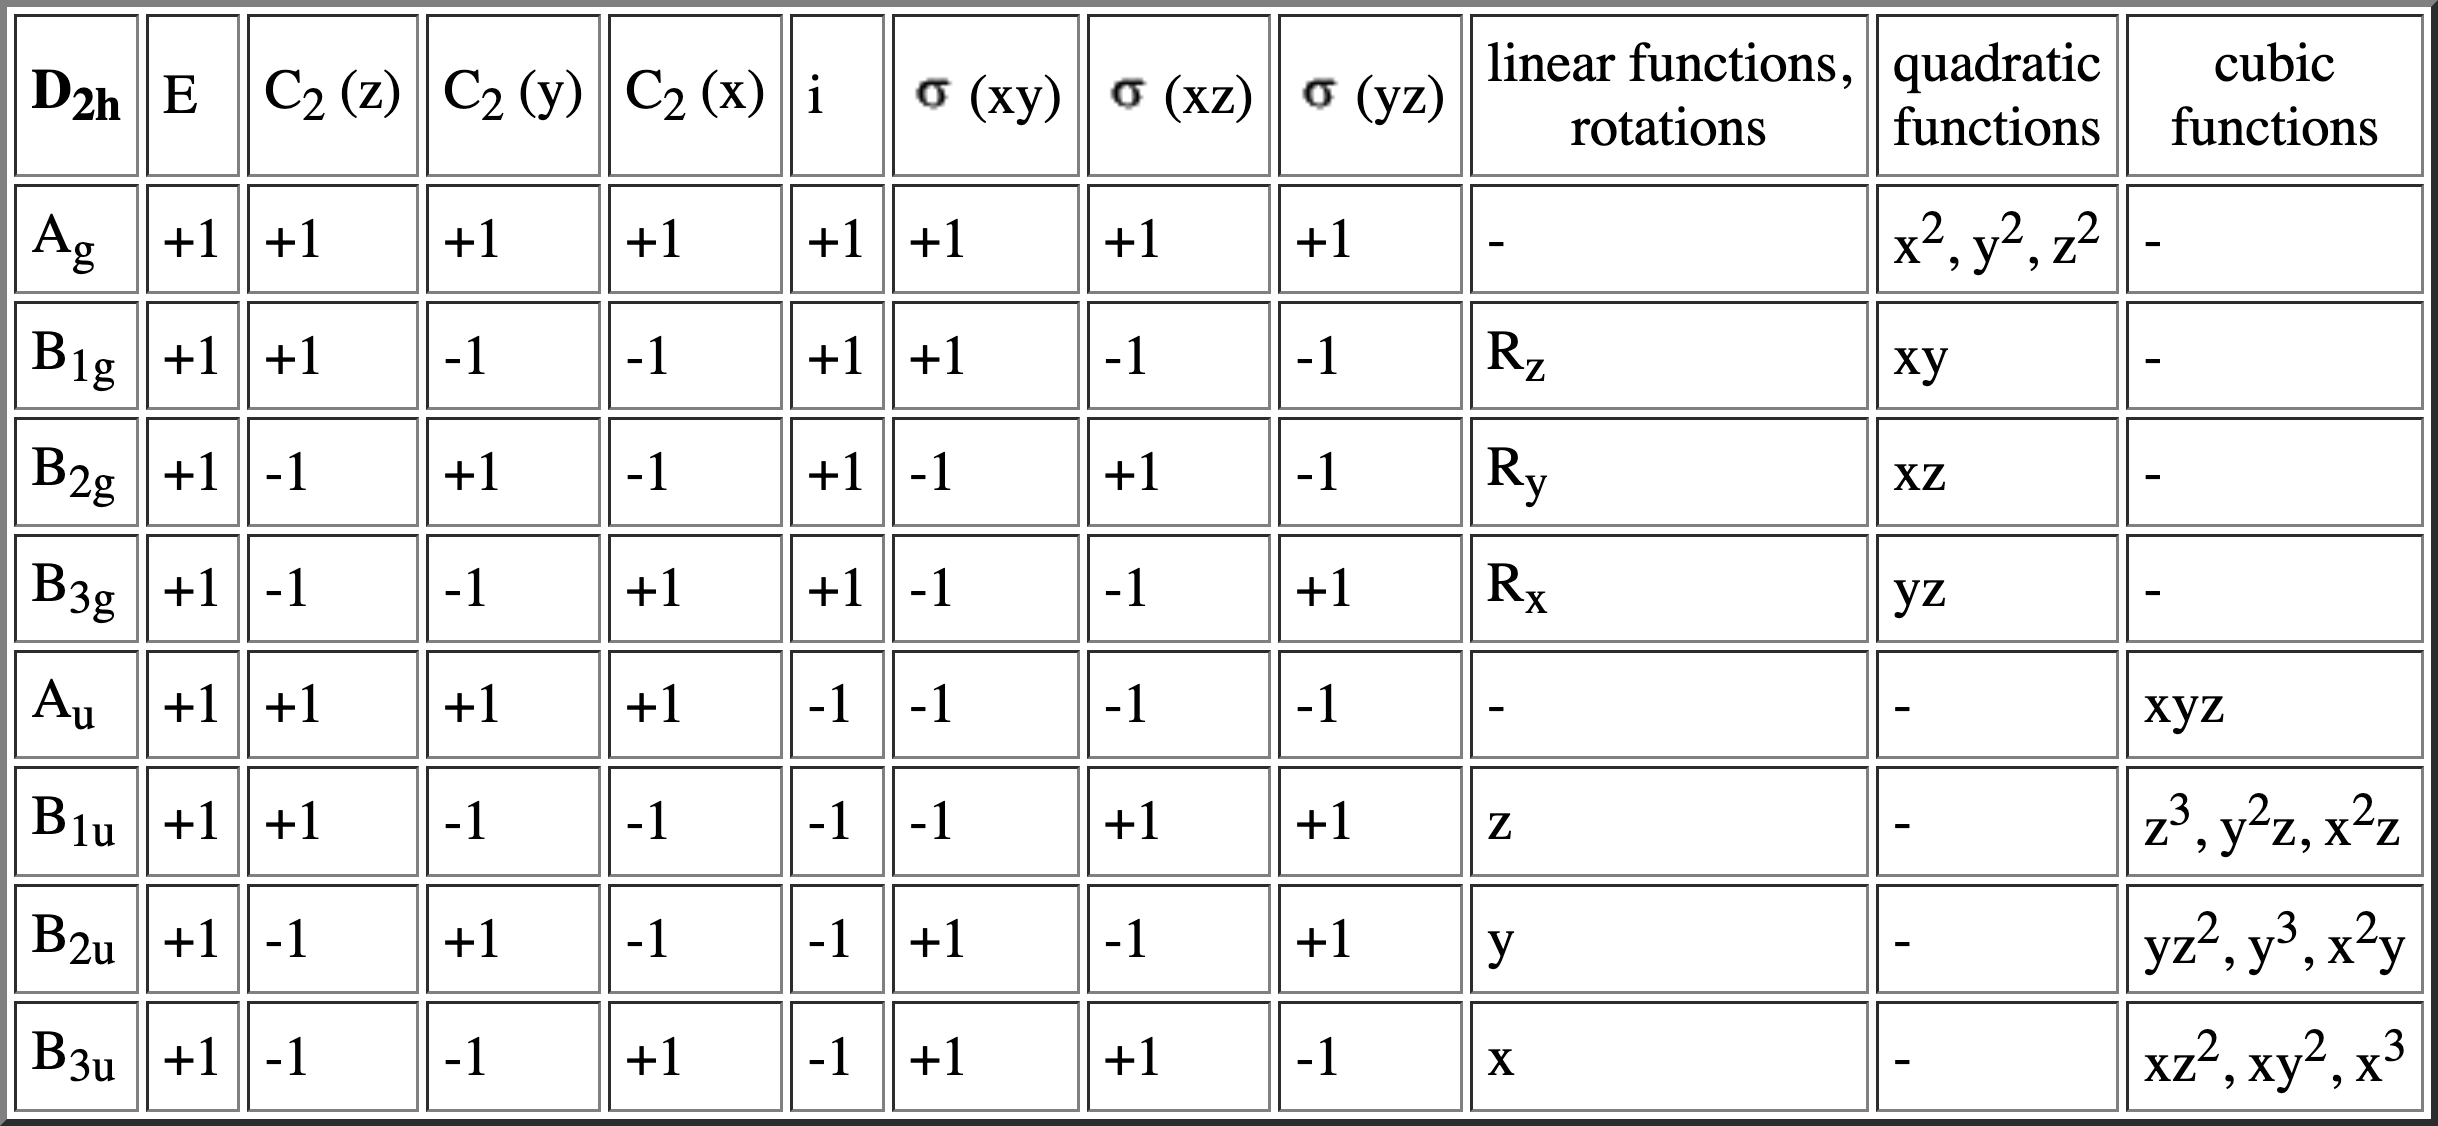
\includegraphics[width=0.8\linewidth]{../ExtFiles/charTableD2h.png}
            \caption{$D_{2h}$ character table.}
            \label{tab:charTableD2h}
        \end{table}
        \item $xyz$ coordinates are chosen as per Figure \ref{fig:xyzCO2}.
        \begin{figure}[h!]
            \centering
            \footnotesize
            \begin{tikzpicture}
                \node{
                    \chemfig{O=@{C}C=@{O}O}
                    \chemmove{
                        \draw [-latex,shorten <=2pt] (O) -- ++(0.7,0,0) node[right]{$z$};
                        \draw [-latex,shorten <=2pt] (C) -- ++(0,0.7,0) node[above]{$x$};
                        \draw [-latex,shorten <=2pt] (C) -- ++(0,0,1.2) node[below left=-2pt]{$y$};
                    }
                };
                \path (-1.1,-0.75) rectangle (1.85,1);
            \end{tikzpicture}
            \caption{\ce{CO2} $xyz$ coordinates.}
            \label{fig:xyzCO2}
        \end{figure}
        \item The two oxygen atoms are peripheral; their valence orbitals are $2s$, $2p_x$, $2p_y$, and $2p_z$. Thus, we have from the $D_{2h}$ character table and Figure \ref{fig:xyzCO2} that
        \begin{table}[h!]
            \centering
            \small
            \renewcommand{\arraystretch}{1.2}
            \begin{tabular}{c|cccccccc}
                $D_{2h}$ & $E$ & $C_2(z)$ & $C_2(y)$ & $C_2(x)$ & $i$ & $\sigma(xy)$ & $\sigma(xz)$ & $\sigma(yz)$\\
                \hline
                $\Gamma_{\ce{O}(2s)}$ & 2 & 2 & 0 & 0 & 0 & 0 & 2 & 2\\
                $\Gamma_{\ce{O}(2p_z)}$ & 2 & 2 & 0 & 0 & 0 & 0 & 2 & 2\\
                $\Gamma_{\ce{O}(2p_x)}$ & 2 & $-2$ & 0 & 0 & 0 & 0 & 2 & $-2$\\
                $\Gamma_{\ce{O}(2p_y)}$ & 2 & $-2$ & 0 & 0 & 0 & 0 & $-2$ & 2\\
            \end{tabular}
            \caption{Representations for the valence orbitals of \ce{CO2}.}
            \label{tab:CO2RR}
        \end{table}
        \begin{itemize}
            \item We get 0 characters for $\Gamma_{\ce{O}(2p_z)}$ because the individual orbitals move, even though the "overall basis" inverts.
        \end{itemize}
        \item As follows.
        \begin{align*}
            \Gamma_{\ce{O}(2s)} = \Gamma_{\ce{O}(2p_z)} &= a_g+b_{1u}\\
            \Gamma_{\ce{O}(2p_x)} &= b_{3u}+b_{2g}\\
            \Gamma_{\ce{O}(2p_y)} &= b_{2u}+b_{3g}
        \end{align*}
        \item Carbon AOs: From the $D_{2h}$ character table,
        \begin{align*}
            \ce{C}(2s) &= a_g&
            \ce{C}(2p_z) &= b_{1u}&
            \ce{C}(2p_x) &= b_{3u}&
            \ce{C}(2p_y) &= b_{2u}
        \end{align*}
        \item We can now construct the following MO diagram.
        \begin{figure}[H]
            \centering
            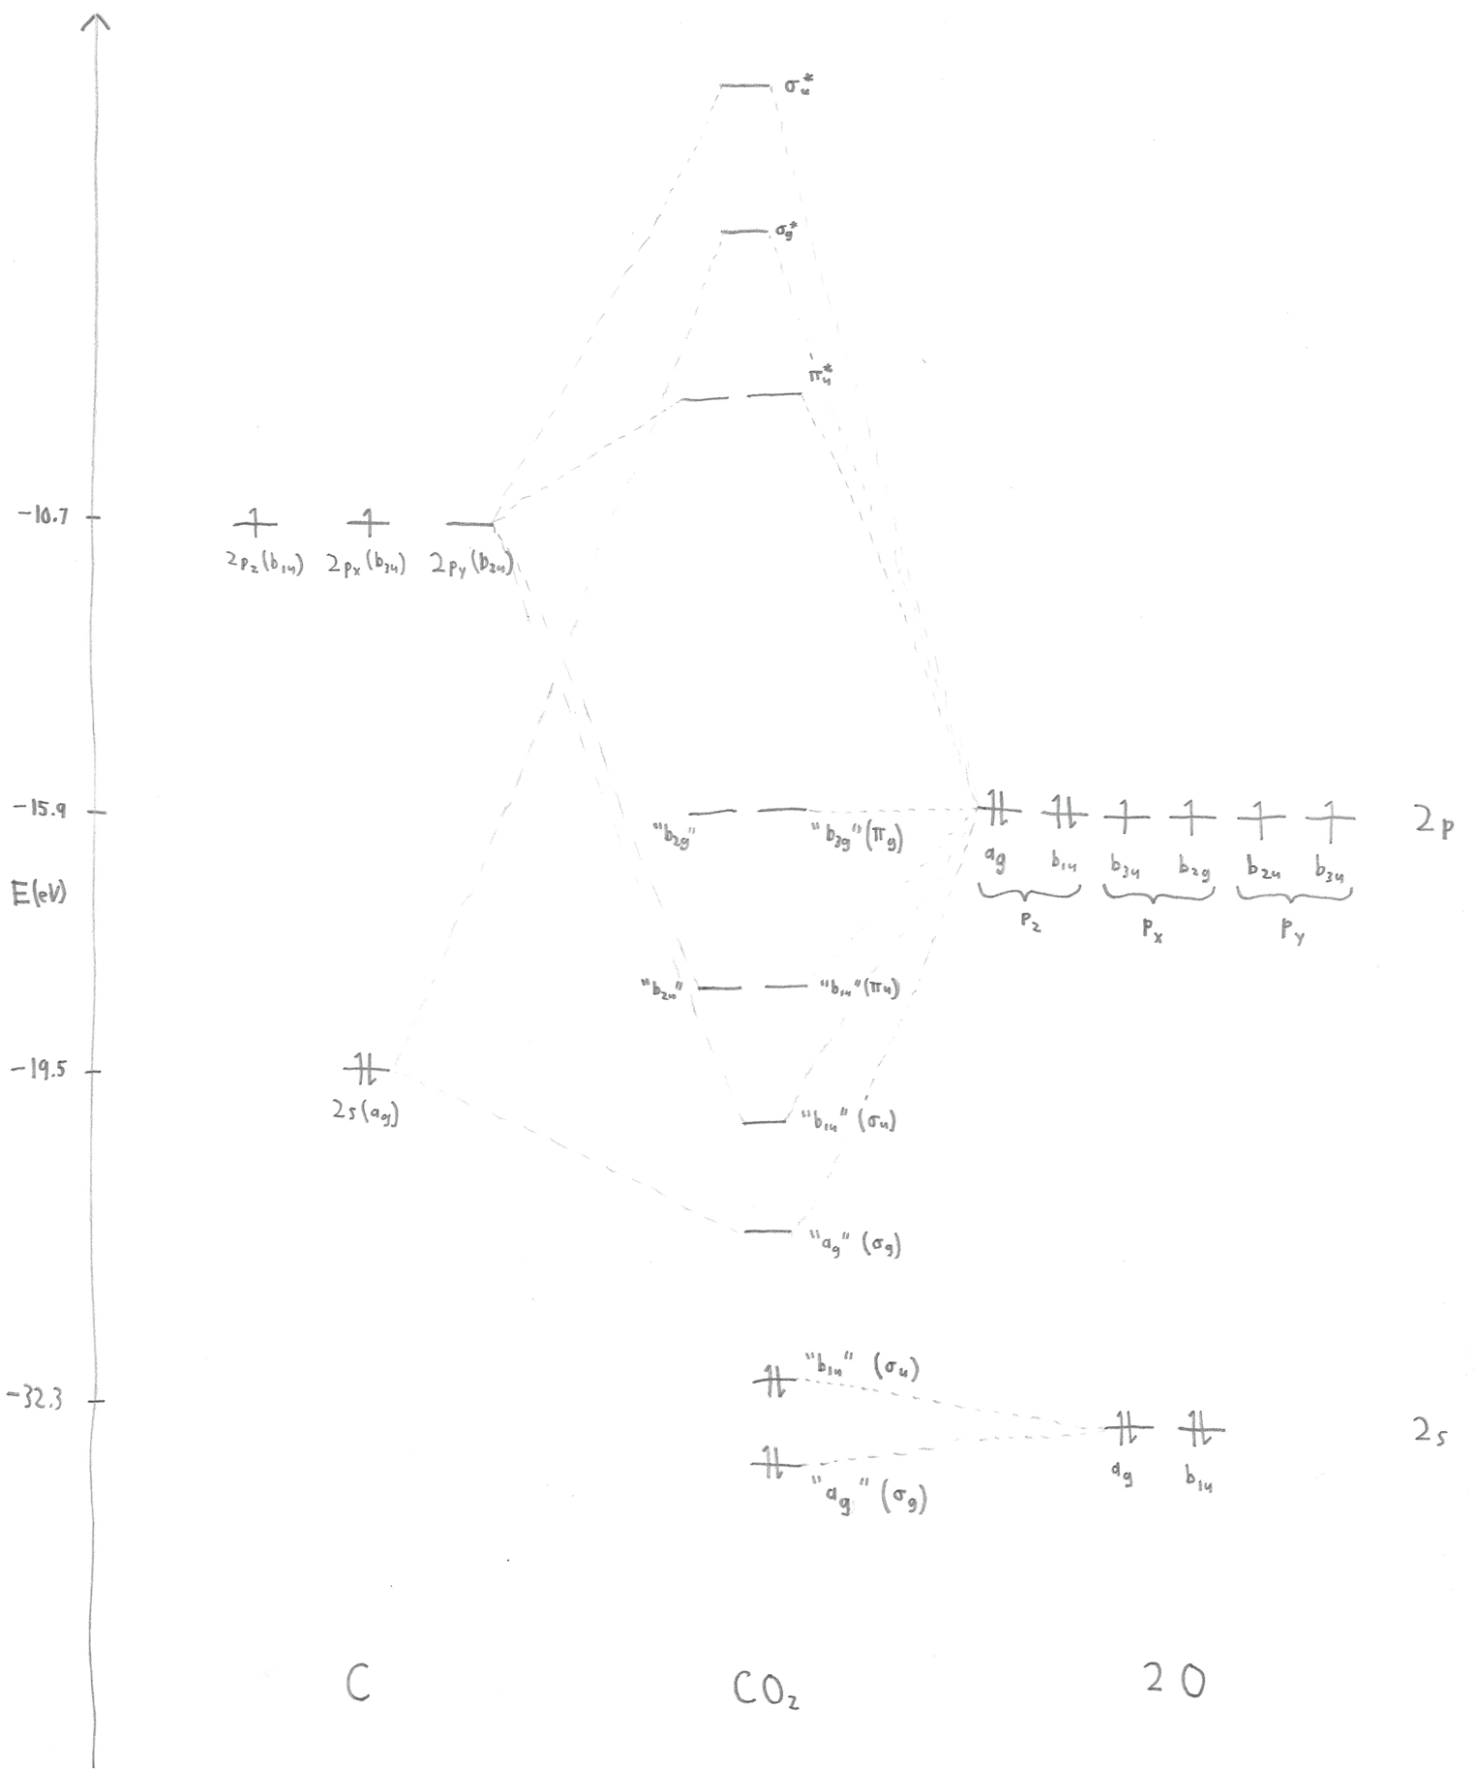
\includegraphics[width=0.7\linewidth]{../ExtFiles/MOsCO2.png}
            \caption{\ce{CO2} MO diagram.}
            \label{fig:MOsCO2}
        \end{figure}
        Moreover, a selection of key SALCs may be visualized as follows.
        \begin{figure}[H]
            \centering
            \begin{subfigure}[b]{0.49\linewidth}
                \centering
                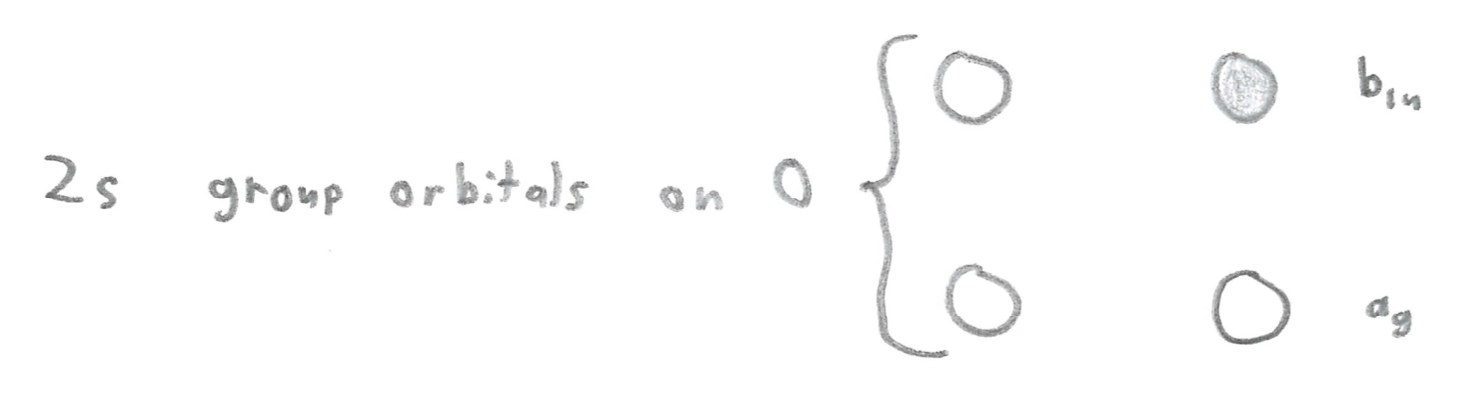
\includegraphics[width=0.8\linewidth]{../ExtFiles/CO2SALCa.png}
                \caption{$\ce{O}(2s)$.}
                \label{fig:CO2SALCa}
            \end{subfigure}
            \begin{subfigure}[b]{0.49\linewidth}
                \centering
                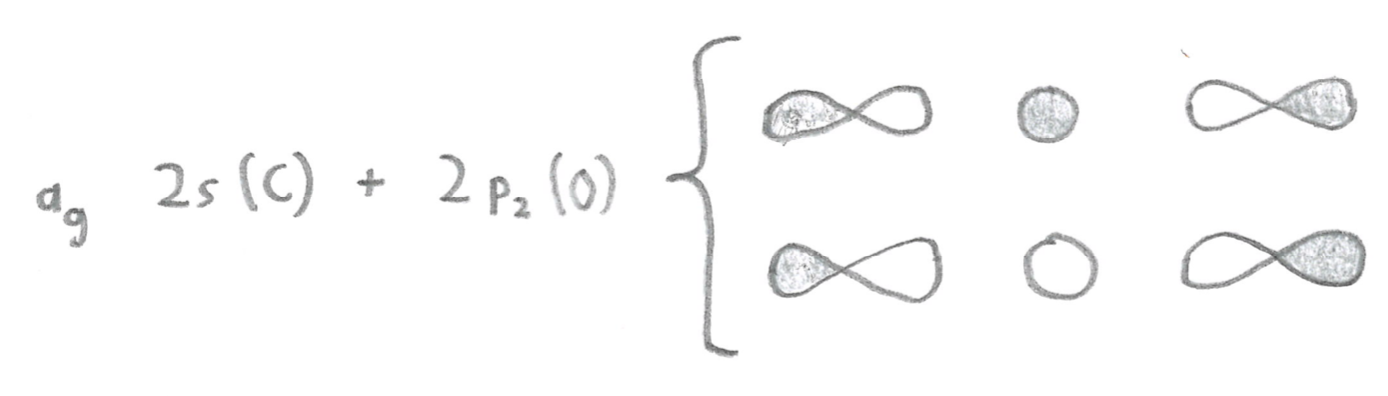
\includegraphics[width=0.8\linewidth]{../ExtFiles/CO2SALCb.png}
                \caption{$a_g$.}
                \label{fig:CO2SALCb}
            \end{subfigure}
        \end{figure}
        \begin{figure}[H]
            \ContinuedFloat
            \centering
            \begin{subfigure}[b]{0.49\linewidth}
                \centering
                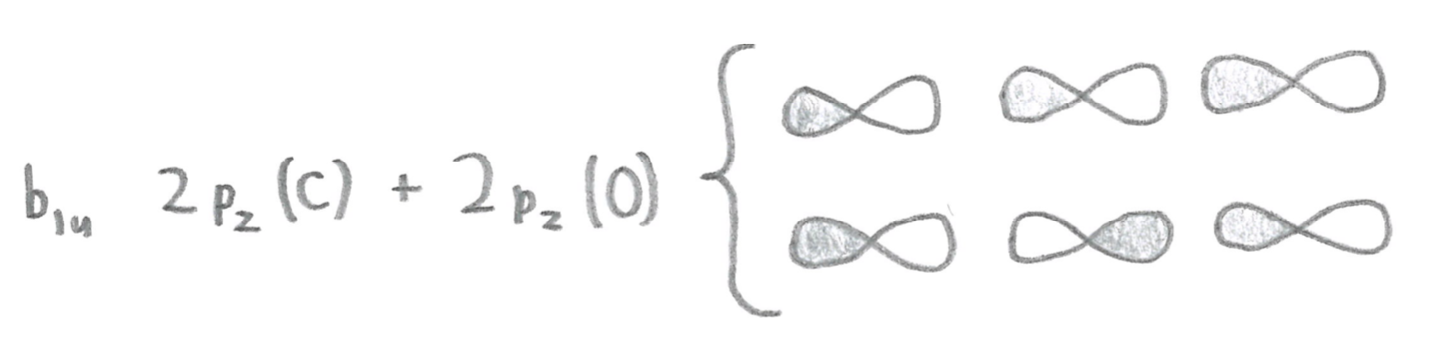
\includegraphics[width=0.8\linewidth]{../ExtFiles/CO2SALCc.png}
                \caption{$b_{1u}$.}
                \label{fig:CO2SALCc}
            \end{subfigure}
            \begin{subfigure}[b]{0.49\linewidth}
                \centering
                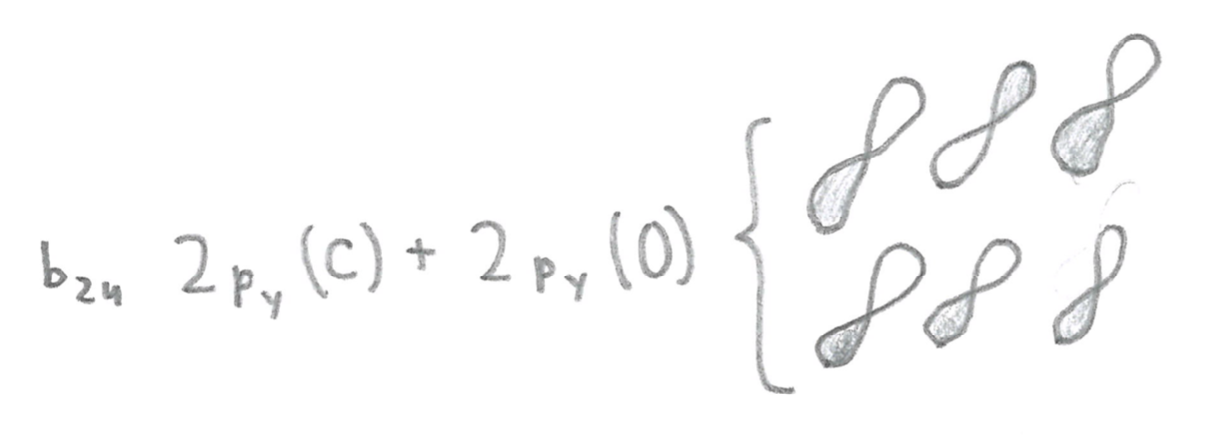
\includegraphics[width=0.8\linewidth]{../ExtFiles/CO2SALCd.png}
                \caption{$b_{2u}$.}
                \label{fig:CO2SALCd}
            \end{subfigure}
            \caption{Selected \ce{CO2} SALCs.}
            \label{fig:CO2SALC}
        \end{figure}
        \begin{itemize}
            \item From the 1 Rydberg rule, oxygen $2s$ orbitals will not significantly overlap with carbon $2s$ or $2p$ orbitals.
            \begin{itemize}
                \item However, we still know that the bonding orbital is slightly lower in energy than the antibonding orbital by counting nodes
                \item A bit of mixing also occurs, though (see the discussion surrounding Figure \ref{fig:calculatedMOsCO2}).
            \end{itemize}
            \item We have so many oxygen electrons since we have \emph{two} oxygens and we are considering their \emph{group} orbitals.
            \item We can draw SALCs intuitively by combining orbitals in a bonding or antibonding fashion, or rigorously using the projection operator.
            \item \emph{Redraw \& add electrons later!}
        \end{itemize}
        \item Done (see Figure \ref{fig:MOsCO2}).
        \item Done (see Figure \ref{fig:MOsCO2}).
    \end{enumerate}
    \item Differences between the \ce{CO2} MOs derived from first principles (Figure \ref{fig:MOsCO2}) and the MOs calculated by a computer's quantum mechanics program (Figure \ref{fig:calculatedMOsCO2}).
    \begin{figure}[H]
        \centering
        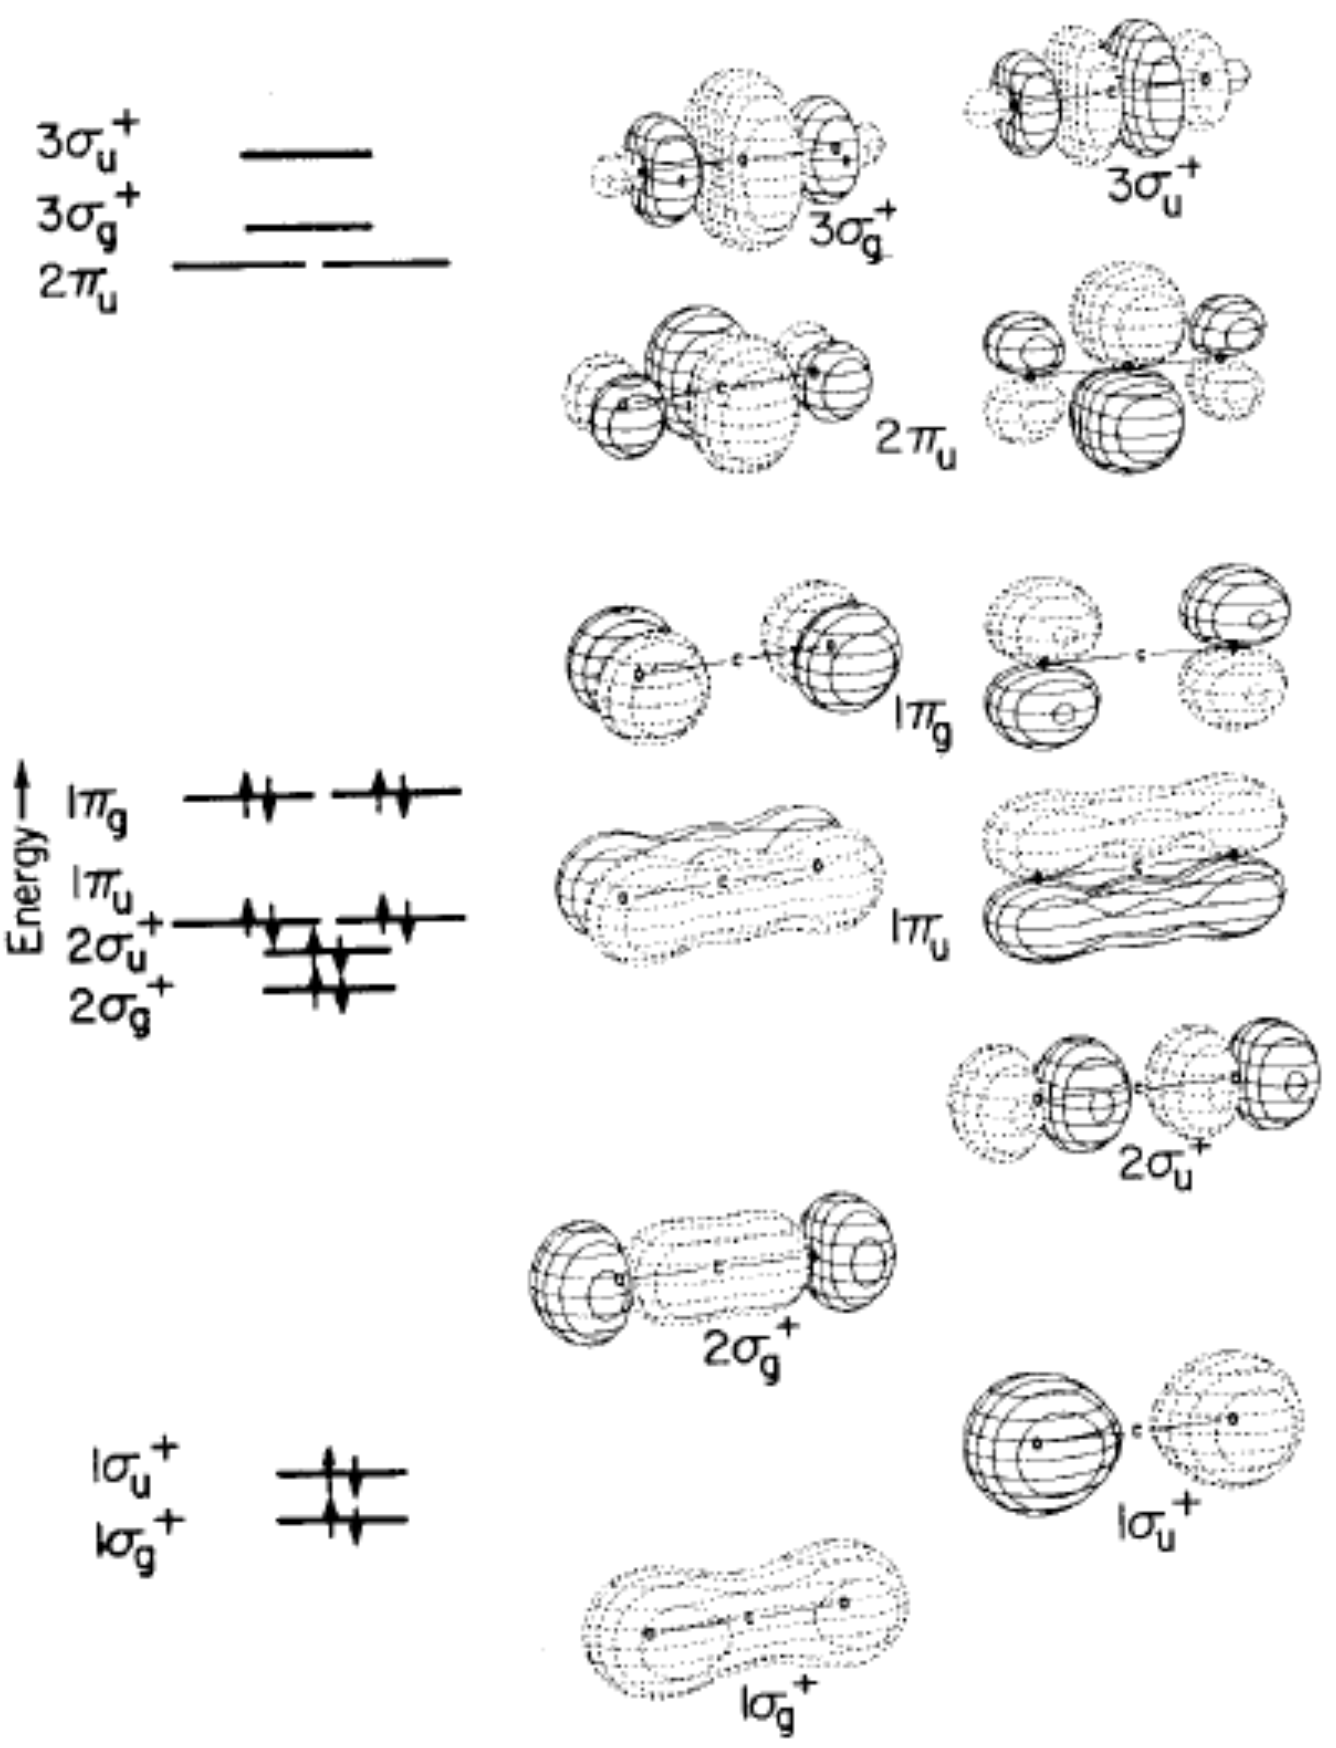
\includegraphics[width=0.5\linewidth]{../ExtFiles/calculatedMOsCO2.png}
        \caption{Quantum-mechanically calculated MOs for \ce{CO2}.}
        \label{fig:calculatedMOsCO2}
    \end{figure}
    \begin{itemize}
        \item In the calculated version, $1\sigma_g$ does not have a node at the carbon atom. This differs from the corresponding SALC we derived from first principles. Thus, in reality, we have some mixing between $1\sigma_g$ and $2\sigma_g$. It follows that we can describe the orbital a bit better as $\ce{O}(2s)$ lone pairs plus \ce{CO} $\sigma$ bonds.
        \item Takeaway: The MOs we get from first principles do not take into account all of the interactions that the computer can.
        \item Note that in Figure \ref{fig:calculatedMOsCO2}, the electron density at each contour surface is \SI[per-mode=symbol]{0.0675}{electrons\per\cubic\angstrom} for one-electron wave functions. This value was chosen merely for satisfactory visual display of the orbitals.
    \end{itemize}
\end{itemize}



\section{Group Orbitals for Nonlinear Molecules}
\begin{itemize}
    \item \marginnote{11/2:}Last time: Making MOs for combinations that have two linear "outer atoms" like \ce{CO2}.
    \item Today: Making MOs for cases in which we can't just add and subtract two valence orbitals to visualize the group orbitals.
    \item Strategy: Make group orbitals for "central atoms" and "peripheral atoms" and combine.
    \item Example: MO diagram for ethylene.
    \begin{enumerate}
        \item Point group: $D_{2h}$.
        \item $xyz$ coordinates (and numbering for the projection operator).
        \begin{figure}[h!]
            \centering
            \begin{tikzpicture}
                \footnotesize
                \node {
                    \chemfig{C_1(-[:120]H_1)(-[:-120]H_3)=C_2(-[:60]H_2)(-[:-60]H_4)}
                };
        
                \draw [-latex] (2,0,0) -- ++(0.7,0,0) node[right]{$x$};
                \draw [-latex] (2,0,0) -- ++(0,0.7,0) node[above]{$y$};
                \draw [-latex] (2,0,0) -- ++(0,0,0.7) node[below left=-2pt]{$z$};
            \end{tikzpicture}
            \caption{\ce{C2H4} $xyz$ coordinates.}
            \label{fig:xyzC2H4}
        \end{figure}
        \item Representations.
        \begin{table}[h!]
            \centering
            \small
            \renewcommand{\arraystretch}{1.2}
            \begin{tabular}{c|cccccccc}
                $D_{2h}$ & $E$ & $C_2(z)$ & $C_2(y)$ & $C_2(x)$ & $i$ & $\sigma(xy)$ & $\sigma(xz)$ & $\sigma(yz)$\\
                \hline
                $\Gamma_{\ce{H}(1s)}$ & 4 & 0 & 0 & 0 & 0 & 4 & 0 & 0\\
                $\Gamma_{\ce{C}(2s)}$ & 2 & 0 & 0 & 2 & 0 & 2 & 2 & 0\\
                $\Gamma_{\ce{C}(2p_x)}$ & 2 & 0 & 0 & 2 & 0 & 2 & 2 & 0\\
                $\Gamma_{\ce{C}(2p_y)}$ & 2 & 0 & 0 & $-2$ & 0 & 2 & $-2$ & 0\\
                $\Gamma_{\ce{C}(2p_z)}$ & 2 & 0 & 0 & $-2$ & 0 & $-2$ & 2 & 0\\
            \end{tabular}
            \caption{Representations for the valence orbitals of \ce{C2H4}.}
            \label{tab:C2H4RR}
        \end{table}
        \item Reductions.
        \begin{align*}
            \Gamma_{\ce{H}(1s)} &= a_g+b_{1g}+b_{2u}+b_{3u}\\
            \Gamma_{\ce{C}(2s)} &= a_g+b_{3u}\\
            \Gamma_{\ce{C}(2p_x)} &= a_g+b_{3u}\\
            \Gamma_{\ce{C}(2p_y)} &= b_{1g}+b_{2u}\\
            \Gamma_{\ce{C}(2p_z)} &= b_{2g}+b_{1u}
        \end{align*}
    \end{enumerate}
    \item Let's get a handle on what some of these orbitals look like using the projection operator.
    \begin{itemize}
        \item Let's see how \ce{H1} and $\ce{C}_{2p_y(1)}$ transform.
        \begin{table}[H]
            \centering
            \small
            \renewcommand{\arraystretch}{1.2}
            \begin{tabular}{c|cccccccc}
                $D_{2h}$ & $E$ & $C_2(z)$ & $C_2(y)$ & $C_2(x)$ & $i$ & $\sigma(xy)$ & $\sigma(xz)$ & $\sigma(yz)$\\
                \hline
                \ce{H1} & \ce{H1} & \ce{H4} & \ce{H2} & \ce{H3} & \ce{H4} & \ce{H1} & \ce{H3} & \ce{H2}\\
                $\ce{C}_{2p_y(1)}$ & $\ce{C}_{2p_y(1)}$ & $-\ce{C}_{2p_y(2)}$ & $\ce{C}_{2p_y(2)}$ & $-\ce{C}_{2p_y(1)}$ & $-\ce{C}_{2p_y(2)}$ & $\ce{C}_{2p_y(1)}$ & $-\ce{C}_{2p_y(1)}$ & $\ce{C}_{2p_y(2)}$\\
            \end{tabular}
            \caption{How selected \ce{C2H4} orbitals transform under the $D_{2h}$ symmetry operations operators.}
            \label{tab:C2H4P}
        \end{table}
        \item We will visualize how these transform under $b_{2u}$. For \ce{H1}, we get
        \begin{align*}
            \hat{P}(\ce{H}_{1s})_{b_{2u}} &= \ce{H1}-\ce{H4}+\ce{H2}-\ce{H3}-\ce{H4}+\ce{H1}-\ce{H3}+\ce{H2}\\
            &= 2\ce{H1}-2\ce{H4}+2\ce{H2}-2\ce{H3}\\
            &\approx \ce{H1}-\ce{H4}+\ce{H2}-\ce{H3}
        \end{align*}
        and for $\ce{C}_{2p_y(1)}$, we get
        \begin{align*}
            \hat{P}(\ce{C}_{2p_y(1)})_{b_{2u}} &= \ce{C}_{2p_y(1)}+\ce{C}_{2p_y(2)}+\ce{C}_{2p_y(2)}+\ce{C}_{2p_y(1)}+\ce{C}_{2p_y(2)}+\ce{C}_{2p_y(1)}+\ce{C}_{2p_y(1)}+\ce{C}_{2p_y(2)}\\
            &= 4(\ce{C}_{2p_y(1)}+\ce{C}_{2p_y(2)})\\
            &\approx \ce{C}_{2p_y(1)}+\ce{C}_{2p_y(2)}
        \end{align*}
        \item Thus, individually, these group orbitals may be visualized as follows.
        \begin{figure}[h!]
            \centering
            \begin{subfigure}[b]{0.3\linewidth}
                \centering
                \begin{tikzpicture}
                    \footnotesize
                    \draw
                        (-1.5em,0) coordinate (C1) -- ++(3em,0) coordinate (C2)
                        (-1.5em,0) ++(120:3em) coordinate (H1) -- (-1.5em,0) -- ++(-120:3em) coordinate (H3)
                        (1.5em,0) ++(60:3em) coordinate (H2) -- (1.5em,0) -- ++(-60:3em) coordinate (H4)
                    ;
        
                    \filldraw [semithick,fill=white] (H1) circle (2.6mm);
                    \filldraw [semithick,fill=white] (H2) circle (2.6mm);
                    \filldraw [semithick,fill=grz] (H3) circle (2.6mm);
                    \filldraw [semithick,fill=grz] (H4) circle (2.6mm);
                \end{tikzpicture}
                \caption{Peripheral atoms.}
                \label{fig:SALCC2H4b2ua}
            \end{subfigure}
            \begin{subfigure}[b]{0.3\linewidth}
                \centering
                \begin{tikzpicture}
                    \footnotesize
                    \draw
                        (-1.5em,0) coordinate (C1) -- ++(3em,0) coordinate (C2)
                        (-1.5em,0) ++(120:3em) coordinate (H1) -- (-1.5em,0) -- ++(-120:3em) coordinate (H3)
                        (1.5em,0) ++(60:3em) coordinate (H2) -- (1.5em,0) -- ++(-60:3em) coordinate (H4)
                    ;
        
                    \filldraw [semithick,fill=white] (C1)
                        to[out=0,in=0,out looseness=0.5] ++(0,0.65)
                        to[out=180,in=180,in looseness=0.5] cycle
                    ;
                    \filldraw [semithick,fill=white] (C2)
                        to[out=0,in=0,out looseness=0.5] ++(0,0.65)
                        to[out=180,in=180,in looseness=0.5] cycle
                    ;
                    \filldraw [semithick,fill=grz] (C1)
                        to[out=0,in=0,out looseness=0.5] ++(0,-0.65)
                        to[out=180,in=180,in looseness=0.5] cycle
                    ;
                    \filldraw [semithick,fill=grz] (C2)
                        to[out=0,in=0,out looseness=0.5] ++(0,-0.65)
                        to[out=180,in=180,in looseness=0.5] cycle
                    ;
                \end{tikzpicture}
                \caption{Central atoms.}
                \label{fig:SALCC2H4b2ub}
            \end{subfigure}
            \caption{\ce{C2H4} $b_{2u}$ SALCs.}
            \label{fig:SALCC2H4b2u}
        \end{figure}
        \item Now we take two orthogonal linear combinations of the two to get our MOs.
        \begin{figure}[h!]
            \centering
            \footnotesize
            \begin{tikzpicture}[
                every node/.style=black
            ]
                \draw [gry,ultra thick]
                    (-2,0) coordinate (H) -- node[below]{$\ce{H}(1s)$} ++(-1.7,0)
                    (2,-1) coordinate (C) -- node[below]{$\ce{C}(2p)$} ++(1.7,0)
                ;
                \draw [ultra thick]
                    (-0.85,1) coordinate (MO2l) -- ++(1.7,0) coordinate (MO2r)
                    (-0.85,-2) coordinate (MO1l) -- ++(1.7,0) coordinate (MO1r)
                ;
        
                \draw [grx,thick,densely dashed]
                    (H) -- (MO2l)
                    (H) -- (MO1l)
                    (C) -- (MO2r)
                    (C) -- (MO1r)
                ;
        
                \begin{scope}[xshift=-2.85cm,yshift=0.8cm,scale=0.6]
                    \draw
                        (-1.5em,0) coordinate (C1) -- ++(3em,0) coordinate (C2)
                        (-1.5em,0) ++(120:3em) coordinate (H1) -- (-1.5em,0) -- ++(-120:3em) coordinate (H3)
                        (1.5em,0) ++(60:3em) coordinate (H2) -- (1.5em,0) -- ++(-60:3em) coordinate (H4)
                    ;
        
                    \filldraw [semithick,fill=white] (H1) circle (2.6mm);
                    \filldraw [semithick,fill=white] (H2) circle (2.6mm);
                    \filldraw [semithick,fill=grz] (H3) circle (2.6mm);
                    \filldraw [semithick,fill=grz] (H4) circle (2.6mm);
                \end{scope}
                \begin{scope}[xshift=2.85cm,yshift=-0.36cm,scale=0.6]
                    \draw
                        (-1.5em,0) coordinate (C1) -- ++(3em,0) coordinate (C2)
                        (-1.5em,0) ++(120:3em) coordinate (H1) -- (-1.5em,0) -- ++(-120:3em) coordinate (H3)
                        (1.5em,0) ++(60:3em) coordinate (H2) -- (1.5em,0) -- ++(-60:3em) coordinate (H4)
                    ;
        
                    \filldraw [semithick,fill=white] (C1)
                        to[out=0,in=0,out looseness=0.5] ++(0,0.65)
                        to[out=180,in=180,in looseness=0.5] cycle
                    ;
                    \filldraw [semithick,fill=white] (C2)
                        to[out=0,in=0,out looseness=0.5] ++(0,0.65)
                        to[out=180,in=180,in looseness=0.5] cycle
                    ;
                    \filldraw [semithick,fill=grz] (C1)
                        to[out=0,in=0,out looseness=0.5] ++(0,-0.65)
                        to[out=180,in=180,in looseness=0.5] cycle
                    ;
                    \filldraw [semithick,fill=grz] (C2)
                        to[out=0,in=0,out looseness=0.5] ++(0,-0.65)
                        to[out=180,in=180,in looseness=0.5] cycle
                    ;
                \end{scope}
                \begin{scope}[xshift=0cm,yshift=1.8cm,scale=0.6]
                    \draw
                        (-1.5em,0) coordinate (C1) -- ++(3em,0) coordinate (C2)
                        (-1.5em,0) ++(120:3em) coordinate (H1) -- (-1.5em,0) -- ++(-120:3em) coordinate (H3)
                        (1.5em,0) ++(60:3em) coordinate (H2) -- (1.5em,0) -- ++(-60:3em) coordinate (H4)
                    ;
        
                    \filldraw [semithick,fill=white] (H1) circle (2.6mm);
                    \filldraw [semithick,fill=white] (H2) circle (2.6mm);
                    \filldraw [semithick,fill=grz] (H3) circle (2.6mm);
                    \filldraw [semithick,fill=grz] (H4) circle (2.6mm);
        
                    \filldraw [semithick,fill=grz] (C1)
                        to[out=0,in=0,out looseness=0.5] ++(0,0.65)
                        to[out=180,in=180,in looseness=0.5] cycle
                    ;
                    \filldraw [semithick,fill=grz] (C2)
                        to[out=0,in=0,out looseness=0.5] ++(0,0.65)
                        to[out=180,in=180,in looseness=0.5] cycle
                    ;
                    \filldraw [semithick,fill=white] (C1)
                        to[out=0,in=0,out looseness=0.5] ++(0,-0.65)
                        to[out=180,in=180,in looseness=0.5] cycle
                    ;
                    \filldraw [semithick,fill=white] (C2)
                        to[out=0,in=0,out looseness=0.5] ++(0,-0.65)
                        to[out=180,in=180,in looseness=0.5] cycle
                    ;
                \end{scope}
                \begin{scope}[xshift=0cm,yshift=-1.2cm,scale=0.6]
                    \draw
                        (-1.5em,0) coordinate (C1) -- ++(3em,0) coordinate (C2)
                        (-1.5em,0) ++(120:3em) coordinate (H1) -- (-1.5em,0) -- ++(-120:3em) coordinate (H3)
                        (1.5em,0) ++(60:3em) coordinate (H2) -- (1.5em,0) -- ++(-60:3em) coordinate (H4)
                    ;
        
                    \filldraw [semithick,fill=white] (H1) circle (2.6mm);
                    \filldraw [semithick,fill=white] (H2) circle (2.6mm);
                    \filldraw [semithick,fill=grz] (H3) circle (2.6mm);
                    \filldraw [semithick,fill=grz] (H4) circle (2.6mm);
        
                    \filldraw [semithick,fill=white] (C1)
                        to[out=0,in=0,out looseness=0.5] ++(0,0.65)
                        to[out=180,in=180,in looseness=0.5] cycle
                    ;
                    \filldraw [semithick,fill=white] (C2)
                        to[out=0,in=0,out looseness=0.5] ++(0,0.65)
                        to[out=180,in=180,in looseness=0.5] cycle
                    ;
                    \filldraw [semithick,fill=grz] (C1)
                        to[out=0,in=0,out looseness=0.5] ++(0,-0.65)
                        to[out=180,in=180,in looseness=0.5] cycle
                    ;
                    \filldraw [semithick,fill=grz] (C2)
                        to[out=0,in=0,out looseness=0.5] ++(0,-0.65)
                        to[out=180,in=180,in looseness=0.5] cycle
                    ;
                \end{scope}
            \end{tikzpicture}
            \caption{\ce{C2H4} $b_{2u}$ MOs.}
            \label{fig:MOsC2H4b2u}
        \end{figure}
        \begin{itemize}
            \item Note that we label the MOs by comparing to the computed orbitals in Figure \ref{fig:calculatedMOsC2H4}.
            \begin{figure}[H]
                \centering
                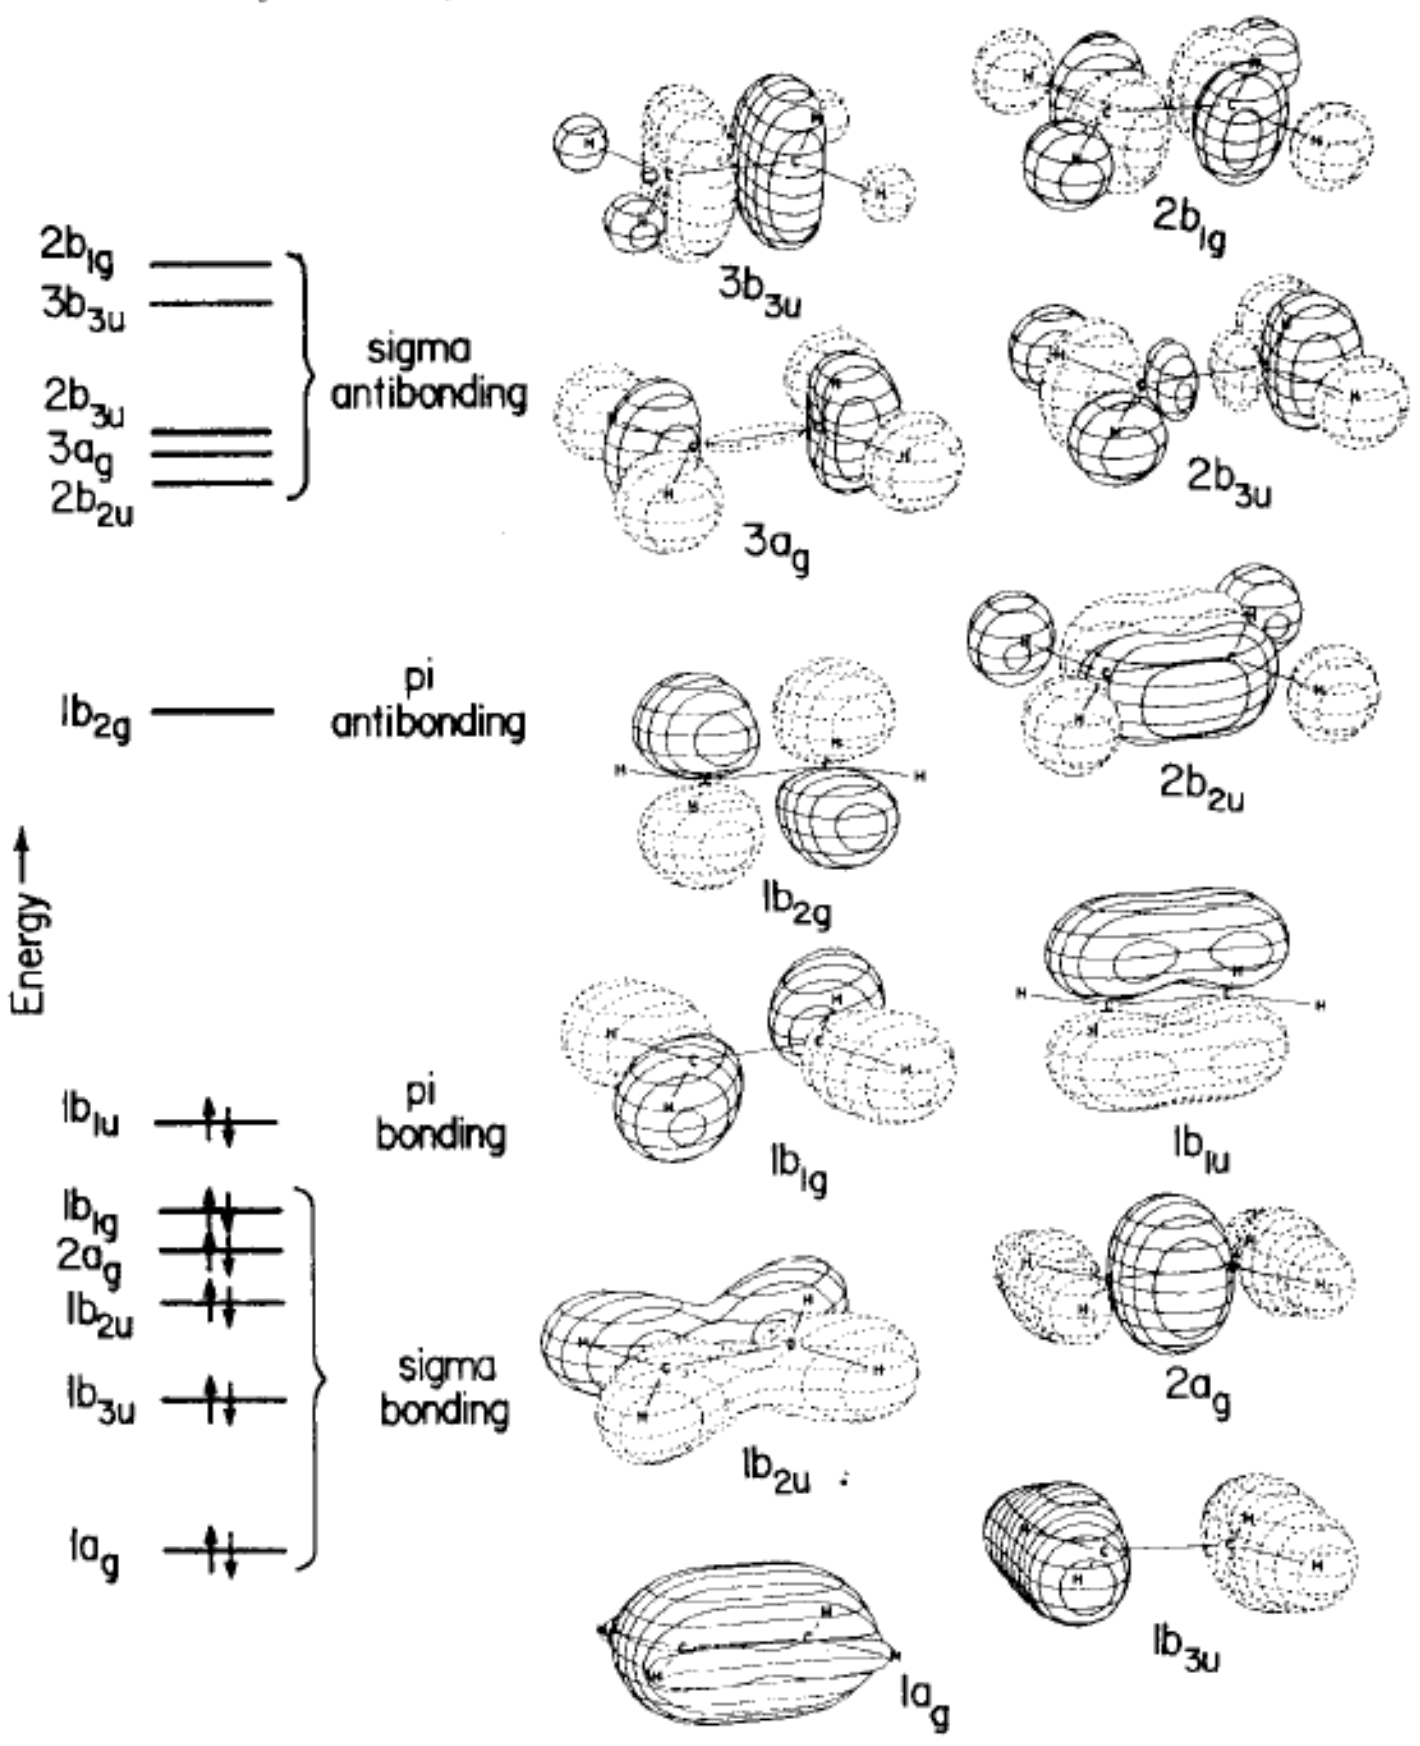
\includegraphics[width=0.45\linewidth]{../ExtFiles/calculatedMOsC2H4.png}
                \caption{Quantum-mechanically calculated MOs for \ce{C2H4}.}
                \label{fig:calculatedMOsC2H4}
            \end{figure}
        \end{itemize}
    \end{itemize}
    \item What about how we make MOs for group orbitals that transform with $e$ symmetry?
    \item Example: Methyl cation.
    \begin{enumerate}
        \item Point group: $D_{3h}$.
        \begin{table}[h!]
            \centering
            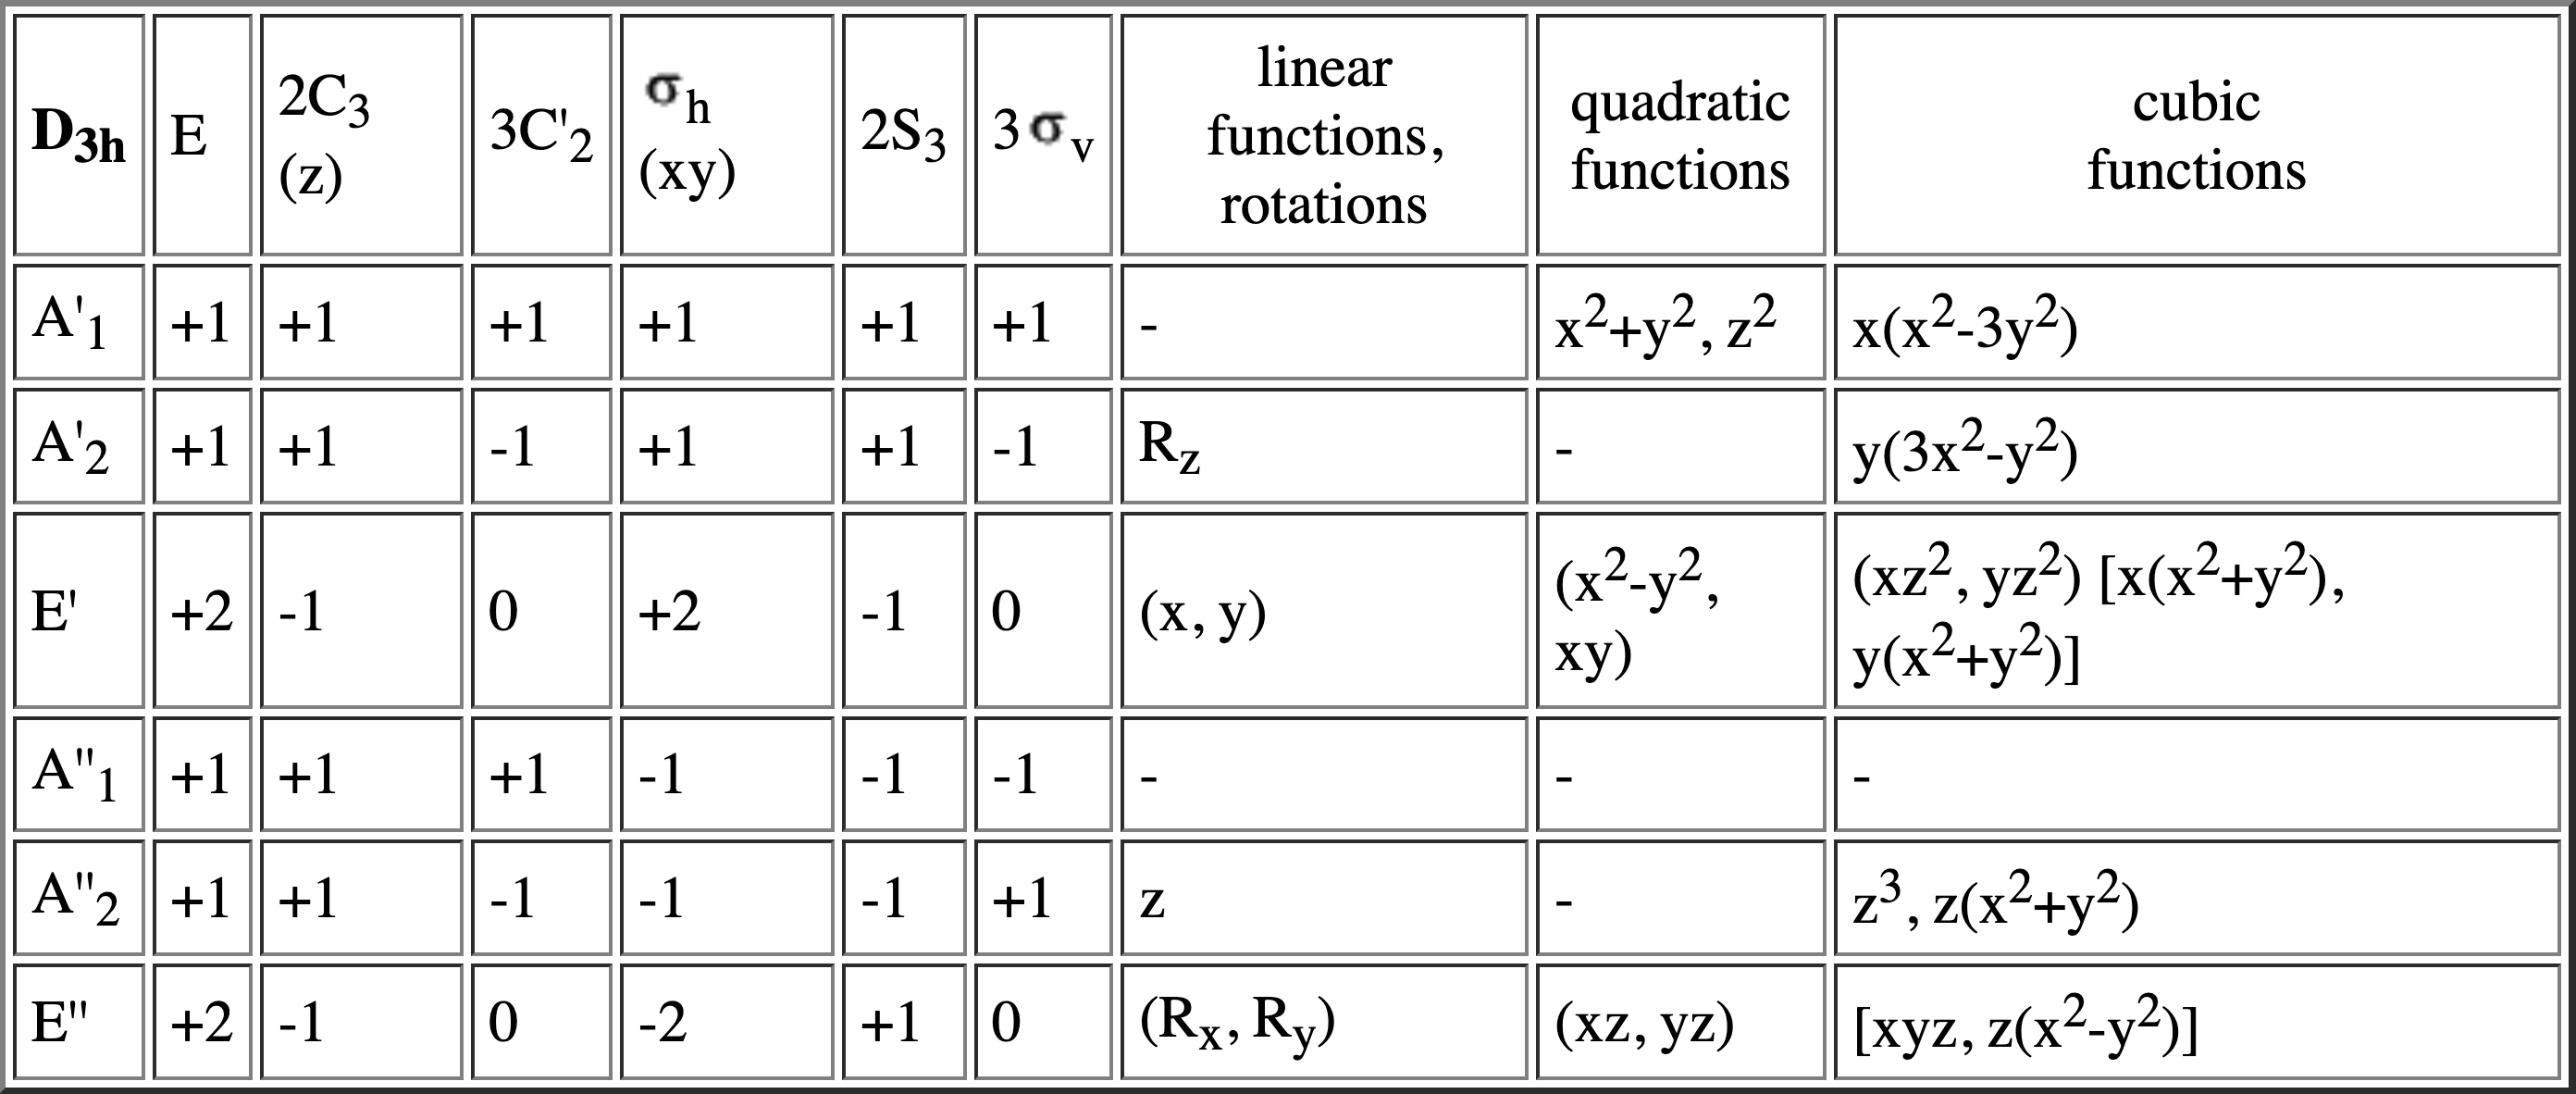
\includegraphics[width=0.8\linewidth]{../ExtFiles/charTableD3h.png}
            \caption{$D_{3h}$ character table.}
            \label{tab:charTableD3h}
        \end{table}
        \item $xyz$ coordinates.
        \begin{figure}[H]
            \centering
            \begin{tikzpicture}
                \footnotesize
                \node {
                    \chemfig{\charge{45:3pt=$\oplus$}{C}(-[:120]H_2)(-H_1)(-[:-120]H_3)}
                };
        
                \draw [-latex] (2,0,0) -- ++(0.7,0,0) node[right]{$x$};
                \draw [-latex] (2,0,0) -- ++(0,0.7,0) node[above]{$y$};
                \draw [-latex] (2,0,0) -- ++(0,0,0.7) node[below left=-2pt]{$z$};
            \end{tikzpicture}
            \caption{\ce{CH3+} $xyz$ coordinates.}
            \label{fig:xyzCH3}
        \end{figure}
        \item Representations.
        \begin{table}[H]
            \centering
            \small
            \renewcommand{\arraystretch}{1.2}
            \begin{tabular}{c|cccccc}
                $D_{3h}$ & $E$ & $2C_3$ & $3C_2$ & $\sigma_h$ & $2S_3$ & $3\sigma_v$\\
                \hline
                $\Gamma_{\ce{H}(1s)}$ & 3 & 0 & 1 & 3 & 0 & 1\\
                $\Gamma_{\ce{C}(2s)}$ & 1 & 1 & 1 & 1 & 1 & 1\\
                $\Gamma_{\ce{C}(2p_x,2p_y)}$ & 2 & $-1$ & 0 & 2 & $-1$ & 0\\
                $\Gamma_{\ce{C}(2p_z)}$ & 1 & 1 & $-1$ & $-1$ & $-1$ & 1\\
            \end{tabular}
            \caption{Representations for the valence orbitals of \ce{CH3+}.}
            \label{tab:CH3RR}
        \end{table}
        \item Reductions.
        \begin{align*}
            \Gamma_{\ce{H}(1s)} &= a_1'+e'\\
            \Gamma_{\ce{C}(2s)} &= a_1'\\
            \Gamma_{\ce{C}(2p_x,2p_y)} &= e'\\
            \Gamma_{\ce{C}(2p_z)} &= a_2''
        \end{align*}
    \end{enumerate}
    \item The projection operator is only necessary for what group orbitals look like.
    \begin{itemize}
        \item How hydrogen orbitals transforms.
        \begin{table}[h!]
            \centering
            \small
            \renewcommand{\arraystretch}{1.2}
            \begin{tabular}{c|cccccccccccc}
                $D_{3h}$ & $E$ & $C_3$ & $C_3^2$ & $C_2$ & $C_2'$ & $C_2''$ & $\sigma_h$ & $S_3$ & $S_3^{-1}$ & $\sigma_v$ & $\sigma_v'$ & $\sigma_v''$\\
                \hline
                \ce{H1} & \ce{H1} & \ce{H2} & \ce{H3} & \ce{H1} & \ce{H3} & \ce{H2} & \ce{H1} & \ce{H2} & \ce{H3} & \ce{H1} & \ce{H2} & \ce{H3}\\
                \ce{H2} & \ce{H2} & \ce{H3} & \ce{H1} & \ce{H2} & \ce{H1} & \ce{H3} & \ce{H2} & \ce{H3} & \ce{H1} & \ce{H2} & \ce{H3} & \ce{H1}\\
                \ce{H3} & \ce{H3} & \ce{H1} & \ce{H2} & \ce{H3} & \ce{H2} & \ce{H1} & \ce{H3} & \ce{H1} & \ce{H2} & \ce{H3} & \ce{H1} & \ce{H2}\\
            \end{tabular}
            \caption{How selected \ce{CH3+} orbitals transform under the $D_{3h}$ symmetry operations operators.}
            \label{tab:CH3P}
        \end{table}
        \item Transformations under $e'$.
        \begin{align*}
            \hat{P}(\ce{H1})_{e'} &\approx 2\ce{H1}-\ce{H2}-\ce{H3}\\
            \hat{P}(\ce{H2})_{e'} &\approx 2\ce{H2}-\ce{H3}-\ce{H1}\\
            \hat{P}(\ce{H3})_{e'} &\approx 2\ce{H3}-\ce{H1}-\ce{H2}
        \end{align*}
        \item We take the first and subtract the second two to get $\ce{H2}-\ce{H3}$ as our second orthogonal orbital.
        \item To draw MOs, we either pair $\ce{C}_{2p_x}$ with $2\ce{H1}-\ce{H2}-\ce{H3}$ and $\ce{C}_{2p_y}$ with $\ce{H2}-\ce{H3}$ or vice versa.
        \begin{figure}[h!]
            \centering
            \footnotesize
            \begin{tikzpicture}[
                every node/.style=black
            ]
                \draw [gry,ultra thick]
                    (-3,0) coordinate (H) -- ++(-1.7,0) ++(-0.1,0) node[below,xshift=-0.5mm]{$\ce{H}(1s)$} -- ++(-1.7,0)
                    (3,-1) coordinate (C) -- node[below]{$\ce{C}(2p_x)$} ++(1.7,0) ++(0.1,0) -- node[below]{$\ce{C}(2p_y)$} ++(1.7,0)
                ;
                \draw [ultra thick]
                    (-1.75,1) coordinate (MO2l) -- ++(1.7,0) ++(0.1,0) -- ++(1.7,0) coordinate (MO2r)
                    (-1.75,-2) coordinate (MO1l) -- ++(1.7,0) ++(0.1,0) -- ++(1.7,0) coordinate (MO1r)
                ;
        
                \draw [grx,thick,densely dashed]
                    (H) -- (MO2l)
                    (H) -- (MO1l)
                    (C) -- (MO2r)
                    (C) -- (MO1r)
                ;
        
                \begin{scope}[xshift=-5.65cm,yshift=0.8cm,scale=0.6,xshift=-0.75em,xshift=1.3mm,yshift=0.92mm]
                    \draw
                        (0,0) coordinate (C) -- ++(120:3em)  coordinate (H2)
                        (0,0)                -- ++(0:3em)    coordinate (H1)
                        (0,0)                -- ++(-120:3em) coordinate (H3)
                    ;
        
                    \filldraw [semithick,fill=white] (H2) circle (2.6mm);
                    \filldraw [semithick,fill=grz] (H3) circle (2.6mm);
                \end{scope}
                \begin{scope}[xshift=-3.85cm,yshift=0.8cm,scale=0.6,xshift=-0.75em,xshift=-0.92mm]
                    \draw
                        (0,0) coordinate (C) -- ++(120:3em)  coordinate (H2)
                        (0,0)                -- ++(0:3em)    coordinate (H1)
                        (0,0)                -- ++(-120:3em) coordinate (H3)
                    ;
        
                    \filldraw [semithick,fill=white] (H1) circle (3.67mm);
                    \filldraw [semithick,fill=grz] (H2) circle (1.84mm);
                    \filldraw [semithick,fill=grz] (H3) circle (1.84mm);
                \end{scope}
                \begin{scope}[xshift=3.85cm,yshift=-0.2cm,scale=0.6,xshift=-0.75em,yshift=-0.92mm]
                    \draw
                        (0,0) coordinate (C) -- ++(120:3em)  coordinate (H2)
                        (0,0)                -- ++(0:3em)    coordinate (H1)
                        (0,0)                -- ++(-120:3em) coordinate (H3)
                    ;
        
                    \filldraw [semithick,fill=white] (C)
                        to[out=90,in=90,out looseness=0.5] ++(0.65,0)
                        to[out=-90,in=-90,in looseness=0.5] cycle
                    ;
                    \filldraw [semithick,fill=grz] (C)
                        to[out=90,in=90,out looseness=0.5] ++(-0.65,0)
                        to[out=-90,in=-90,in looseness=0.5] cycle
                    ;
                \end{scope}
                \begin{scope}[xshift=5.65cm,yshift=-0.2cm,scale=0.6,xshift=-0.75em,yshift=-0.92mm]
                    \draw
                        (0,0) coordinate (C) -- ++(120:3em)  coordinate (H2)
                        (0,0)                -- ++(0:3em)    coordinate (H1)
                        (0,0)                -- ++(-120:3em) coordinate (H3)
                    ;
        
                    \filldraw [semithick,fill=white] (C)
                        to[out=0,in=0,out looseness=0.5] ++(0,0.65)
                        to[out=180,in=180,in looseness=0.5] cycle
                    ;
                    \filldraw [semithick,fill=grz] (C)
                        to[out=0,in=0,out looseness=0.5] ++(0,-0.65)
                        to[out=180,in=180,in looseness=0.5] cycle
                    ;
                \end{scope}
                \begin{scope}[xshift=-0.9cm,yshift=1.8cm,scale=0.6,xshift=-0.75em,xshift=1.3mm,yshift=0.92mm]
                    \draw
                        (0,0) coordinate (C) -- ++(120:3em)  coordinate (H2)
                        (0,0)                -- ++(0:3em)    coordinate (H1)
                        (0,0)                -- ++(-120:3em) coordinate (H3)
                    ;
        
                    \filldraw [semithick,fill=white] (H2) circle (2.6mm);
                    \filldraw [semithick,fill=grz] (H3) circle (2.6mm);
        
                    \filldraw [semithick,fill=grz] (C)
                        to[out=0,in=0,out looseness=0.5] ++(0,0.65)
                        to[out=180,in=180,in looseness=0.5] cycle
                    ;
                    \filldraw [semithick,fill=white] (C)
                        to[out=0,in=0,out looseness=0.5] ++(0,-0.65)
                        to[out=180,in=180,in looseness=0.5] cycle
                    ;
                \end{scope}
                \begin{scope}[xshift=0.9cm,yshift=1.8cm,scale=0.6,xshift=-0.75em,xshift=-0.92mm]
                    \draw
                        (0,0) coordinate (C) -- ++(120:3em)  coordinate (H2)
                        (0,0)                -- ++(0:3em)    coordinate (H1)
                        (0,0)                -- ++(-120:3em) coordinate (H3)
                    ;
        
                    \filldraw [semithick,fill=white] (H1) circle (3.67mm);
                    \filldraw [semithick,fill=grz] (H2) circle (1.84mm);
                    \filldraw [semithick,fill=grz] (H3) circle (1.84mm);
        
                    \filldraw [semithick,fill=grz] (C)
                        to[out=90,in=90,out looseness=0.5] ++(0.65,0)
                        to[out=-90,in=-90,in looseness=0.5] cycle
                    ;
                    \filldraw [semithick,fill=white] (C)
                        to[out=90,in=90,out looseness=0.5] ++(-0.65,0)
                        to[out=-90,in=-90,in looseness=0.5] cycle
                    ;
                \end{scope}
                \begin{scope}[xshift=-0.9cm,yshift=-1.2cm,scale=0.6,xshift=-0.75em,xshift=1.3mm,yshift=0.92mm]
                    \draw
                        (0,0) coordinate (C) -- ++(120:3em)  coordinate (H2)
                        (0,0)                -- ++(0:3em)    coordinate (H1)
                        (0,0)                -- ++(-120:3em) coordinate (H3)
                    ;
        
                    \filldraw [semithick,fill=white] (H2) circle (2.6mm);
                    \filldraw [semithick,fill=grz] (H3) circle (2.6mm);
        
                    \filldraw [semithick,fill=white] (C)
                        to[out=0,in=0,out looseness=0.5] ++(0,0.65)
                        to[out=180,in=180,in looseness=0.5] cycle
                    ;
                    \filldraw [semithick,fill=grz] (C)
                        to[out=0,in=0,out looseness=0.5] ++(0,-0.65)
                        to[out=180,in=180,in looseness=0.5] cycle
                    ;
                \end{scope}
                \begin{scope}[xshift=0.9cm,yshift=-1.2cm,scale=0.6,xshift=-0.75em,xshift=-0.92mm]
                    \draw
                        (0,0) coordinate (C) -- ++(120:3em)  coordinate (H2)
                        (0,0)                -- ++(0:3em)    coordinate (H1)
                        (0,0)                -- ++(-120:3em) coordinate (H3)
                    ;
        
                    \filldraw [semithick,fill=white] (H1) circle (3.67mm);
                    \filldraw [semithick,fill=grz] (H2) circle (1.84mm);
                    \filldraw [semithick,fill=grz] (H3) circle (1.84mm);
        
                    \filldraw [semithick,fill=white] (C)
                        to[out=90,in=90,out looseness=0.5] ++(0.65,0)
                        to[out=-90,in=-90,in looseness=0.5] cycle
                    ;
                    \filldraw [semithick,fill=grz] (C)
                        to[out=90,in=90,out looseness=0.5] ++(-0.65,0)
                        to[out=-90,in=-90,in looseness=0.5] cycle
                    ;
                \end{scope}
            \end{tikzpicture}
            \caption{\ce{CH3+} $e'$ MOs.}
            \label{fig:MOsCH3e}
        \end{figure}
        \begin{itemize}
            \item Note that the two bonding and the two antibonding MOs here are pairwise degenerate.
        \end{itemize}
    \end{itemize}
    \item Should we label the MOs via PES as in CHEM 201?
    \begin{itemize}
        \item Yes.
    \end{itemize}
    \item Finding energies from SALCs?
\end{itemize}



\section{Photoelectron Spectroscopy and MO Diagrams of Coordination Complexes}
\begin{itemize}
    \item \marginnote{11/4:}The problem set is deceptively hard; get started early!
    \item Today: Experimental verification of molecular orbitals.
    \item \textbf{Photoelectron spectroscopy}: A widely used technique that allows us to obtain information about the energies of the electrons in orbitals.
    \item Key equation.
    \begin{equation*}
        \text{BE} = h\nu-\text{KE}
    \end{equation*}
    \begin{itemize}
        \item $\text{BE}$ is the binding energy of the expelled electron.
        \item $h\nu$ is the incident photon energy.
        \item $\text{KE}$ is the kinetic energy of the expelled electron.
    \end{itemize}
    \item Fine structure in PES comes from the interaction of the electronic levels with the vibrational levels. This yields multiple peaks for a single given electronic transition.
    \item Example: How many peaks in the PES should we expect for each occupied MO of ethylene? Label each peak with the relevant valence molecular orbitals for ethylene.
    \begin{figure}[h!]
        \centering
        \begin{tikzpicture}[
            every node/.style=black
        ]
            \small
            \draw (0,3) -- node[rotate=90,above]{Counts per Second} (0,0) -- node[below=3mm]{IE (\si{\electronvolt})} (6,0);
    
            \footnotesize
            \foreach \x in {0.3,0.6,...,5.7} {
                \draw (\x,0) -- ++(0,0.1);
            }
            \node [below] at (0.9,0) {25};
            \node [below] at (2.4,0) {20};
            \node [below] at (3.9,0) {15};
            \node [below] at (5.4,0) {10};
    
            \draw [rex,thick] (0,0.3)
                -- ++(1,0)
                to[out=0,in=180] ++(0.4,0.2) node[above]{$1a_g$}
                to[out=0,in=180] ++(0.2,-0.2)
                -- ++(0.7,0)
                to[out=0,in=-150] ++(0.2,0.3)
                to[out=30,in=180,in looseness=0.7] ++(0.2,0.2) node[above]{$1b_{3u}$}
                to[out=0,in=180,out looseness=0.7] ++(0.2,-0.5)
                -- ++(0.1,0)
                to[out=0,in=180,in looseness=0.2] ++(0.6,1) node[above,xshift=-2mm]{$1b_{2u}$}
                to[out=0,in=180,out looseness=0.2] ++(0.2,-0.3)
                to[out=0,in=-130,out looseness=0.1] ++(0.1,0.2)
                to[out=50,in=180,in looseness=0.2] ++(0.1,0.2) node[above]{$2a_g$}
                to[out=0,in=135] ++(0.1,-0.1)
                to[out=-45,in=180,out looseness=0.2,in looseness=0.2] ++(0.1,-0.8)
                to[out=0,in=180,out looseness=0.8,in looseness=0.1] ++(0.3,0.8) node[above,xshift=1mm]{$1b_{1g}$}
                to[out=0,in=135] ++(0.1,-0.1)
                to[out=-45,in=160,out looseness=0.2,in looseness=0.2] ++(0.1,-0.9)
                to[out=-20,in=180,out looseness=0.6,in looseness=0.03] ++(0.5,2.3) node[above]{$1b_{1u}$}
                to[out=0,in=180,out looseness=0.03,in looseness=0.3] ++(0.2,-2.3)
            ;
        \end{tikzpicture}
        \caption{Photoelectron spectrum of \ce{C2H4}.}
        \label{fig:PESC2H4}
    \end{figure}
    \begin{itemize}
        \item 1 peak for each occupied MO.
        \item Highest IE corresponds to the most core orbital. Decreases in energy as we get to higher energy orbitals.
        \item When Wuttig says in the homework that she wants us to draw a qualitative photoelectron spectrum, this is what she means.
    \end{itemize}
    \item We now translate the principals of MO diagrams we've developed to understand bonding and structure in coordination complexes. We abbreviate the metal as M and the ligand as L.
    \item Basis sets are denoted by $\phi$.
    \item Basis sets.
    \begin{itemize}
        \item M: $(n+1)p$, $(n+1)s$, and $nd$.
        \item L: $\sigma\to\sigma$ interactions, $\pi\to\pi$ interactions, and $\pi^*\to\pi^*$ interactions.
    \end{itemize}
    \item Today: The $\sigma\to\sigma$ case only.
    \item A few general rules for M-L bonding (these are essentially a rephrasing of those we have developed for the MOs of the organic species we have discussed this far).
    \begin{enumerate}
        \item M-L atomic orbital mixing is proportional to the overlap of the M and L orbitals.
        \begin{enumerate}
            \item But only orbitals of correct symmetry can mix.
            \item $\sigma$ interactions typically give rise to larger interaction energies than $\pi$ interactions which, in turn, typically give rise to larger interaction energies than $\delta$ interactions. This is because we have more directional bonding as we move from $\sigma\to\pi\to\delta$.
        \end{enumerate}
        \item M-L atomic orbital mixing is inversely proportional to energy difference of mixing orbitals.
        \item The order of the $E_{\ce{L}}$ and $E_{\ce{M}}$ energy levels almost always is the following.
        \begin{equation*}
            \sigma(\ce{L}) < \pi(\ce{L})
            < nd
            < (n+1)s
            < (n+1)p
        \end{equation*}
        \begin{enumerate}
            \item Energy ordering origin: Metal/main group VOIEs and ligand electronic spectra.
        \end{enumerate}
    \end{enumerate}
    \item Impact of VOIE as you move later in the periodic table.
    \begin{itemize}
        \item Metals.
        \begin{itemize}
            \item More covalency with L.
            \item Less $d$-$s$-$p$ mixing.
        \end{itemize}
        \item Common ligands.
        \begin{itemize}
            \item More mixing with lone pairs compared to bonding orbitals.
        \end{itemize}
    \end{itemize}
    \item Conclusions from examining VOIEs.
    \begin{enumerate}
        \item The $s$ orbitals are generally too low in energy to participate in bonding.
        \item The filled $p$ orbitals are the frontier orbitals, and they have VOIEs that place them below metal orbitals.
        \item For ligands, since the frontier orbitals comprise $s$ and $p$ orbitals, filled ligand orbitals have energies $E$ that are stabilized relative to metal orbitals.
    \end{enumerate}
    \item Symmetry.
    \item We will now build the $\sigma$-only MO diagram for the important \ce{ML6} octahedral case.
    \begin{enumerate}
        \item Point group: $O_h$.
        \begin{table}[H]
            \centering
            \small
            \renewcommand{\arraystretch}{1.2}
            \begin{tabular}{l|cccccccccc|l|l}
                $O_h$ & $E$ & $8C_3$ & $6C_2$ & $6C_4$ & $3C_2(={C_4}^2)$ & $i$ & $6S_4$ & $8S_6$ & $3\sigma_h$ & $6\sigma_d$ & linear & quadratic\\
                \hline
                $A_{1g}$ & $1$ & $1$  & $1$  & $1$  & $1$  & $1$  & $1$  & $1$  & $1$  & $1$  & & $x^2+y^2+z^2$\\
                $A_{2g}$ & $1$ & $1$  & $-1$ & $-1$ & $1$  & $1$  & $-1$ & $1$  & $1$  & $-1$ & & \\
                $E_g$    & $2$ & $-1$ & $0$  & $0$  & $2$  & $2$  & $0$  & $-1$ & $2$  & $0$  & & $(2z^2-x^2-y^2,x^2-y^2)$\\
                $T_{1g}$ & $3$ & $0$  & $-1$ & $1$  & $-1$ & $3$  & $1$  & $0$  & $-1$ & $-1$ & $(R_x,R_y,R_z)$ & \\
                $T_{2g}$ & $3$ & $0$  & $1$  & $-1$ & $-1$ & $3$  & $-1$ & $0$  & $-1$ & $1$  & & $(xy,xz,yz)$\\
                $A_{1u}$ & $1$ & $1$  & $1$  & $1$  & $1$  & $-1$ & $-1$ & $-1$ & $-1$ & $-1$ & & \\
                $A_{2u}$ & $1$ & $1$  & $-1$ & $-1$ & $1$  & $-1$ & $1$  & $-1$ & $-1$ & $1$  & & \\
                $E_u$    & $2$ & $-1$ & $0$  & $0$  & $2$  & $-2$ & $0$  & $1$  & $-2$ & $0$  & & \\
                $T_{1u}$ & $3$ & $0$  & $-1$ & $1$  & $-1$ & $-3$ & $-1$ & $0$  & $1$  & $1$  & $(x,y,z)$ & \\
                $T_{2u}$ & $3$ & $0$  & $1$  & $-1$ & $-1$ & $-3$ & $1$  & $0$  & $1$  & $-1$ & & \\
            \end{tabular}
            \caption{Character table for the $O_h$ point group.}
            \label{tab:charTableOh}
        \end{table}
        \item A coordinate system is not particularly necessary here since the molecule is symmetric along every Cartesian axis.
        \item Reducible representation for the $\sigma$ orbitals.
        \begin{table}[H]
            \centering
            \small
            \renewcommand{\arraystretch}{1.2}
            \begin{tabular}{c|cccccccccc}
                $O_h$ & $E$ & $8C_3$ & $6C_2$ & $6C_4$ & $3C_2$ & $i$ & $6S_4$ & $8S_6$ & $3\sigma_h$ & $6\sigma_d$\\
                \hline
                $\Gamma_\sigma$ & 6 & 0 & 0 & 2 & 2 & 0 & 0 & 0 & 4 & 2\\
            \end{tabular}
            \caption{Representation for the $\sigma$ orbitals of \ce{ML6}.}
            \label{tab:ML6RR}
        \end{table}
        \item Reduction.
        \begin{equation*}
            \Gamma_\sigma = a_{1g}+e_g+t_{1u}
        \end{equation*}
        \item Symmetries of the metal atomic orbitals (from Table \ref{tab:charTableOh}).
        \begin{align*}
            s &\sim a_{1g}&
            p_x,p_y,p_z &\sim t_{1u}&
            d_{z^2},d_{x^2-y^2} &\sim e_g&
            d_{xz},d_{yz},d_{xy} &\sim t_{2g}
        \end{align*}
        \item What the SALCs end up looking like.
        \begin{figure}[h!]
            \centering
            \begin{subfigure}[b]{0.24\linewidth}
                \centering
                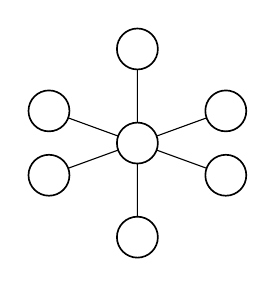
\begin{tikzpicture}
                    \footnotesize
                    \draw
                        (0,0) coordinate (M) -- ++(90:4em)   coordinate (L1)
                        (0,0)                -- ++(-160:4em) coordinate (L2)
                        (0,0)                -- ++(-20:4em)  coordinate (L3)
                        (0,0)                -- ++(20:4em)   coordinate (L4)
                        (0,0)                -- ++(160:4em)  coordinate (L5)
                        (0,0)                -- ++(-90:4em)  coordinate (L6)
                    ;
        
                    \filldraw [semithick,fill=white] (M)  circle (2.6mm);
                    \filldraw [semithick,fill=white] (L1) circle (2.6mm);
                    \filldraw [semithick,fill=white] (L2) circle (2.6mm);
                    \filldraw [semithick,fill=white] (L3) circle (2.6mm);
                    \filldraw [semithick,fill=white] (L4) circle (2.6mm);
                    \filldraw [semithick,fill=white] (L5) circle (2.6mm);
                    \filldraw [semithick,fill=white] (L6) circle (2.6mm);
        
                    \path [semithick] (L6) circle (3.67mm);
                \end{tikzpicture}
                \caption{$a_{1g}$ bonding.}
                \label{fig:SALCML6a}
            \end{subfigure}
            \begin{subfigure}[b]{0.24\linewidth}
                \centering
                \begin{tikzpicture}
                    \footnotesize
                    \draw
                        (0,0) coordinate (M) -- ++(90:4em)   coordinate (L1)
                        (0,0)                -- ++(-160:4em) coordinate (L2)
                        (0,0)                -- ++(-20:4em)  coordinate (L3)
                        (0,0)                -- ++(20:4em)   coordinate (L4)
                        (0,0)                -- ++(160:4em)  coordinate (L5)
                        (0,0)                -- ++(-90:4em)  coordinate (L6)
                    ;
        
                    \filldraw [semithick,fill=white,rotate=-70] (M)
                        to[out=0,in=0,out looseness=0.5] ++(0,0.65)
                        to[out=180,in=180,in looseness=0.5] cycle
                    ;
                    \filldraw [semithick,fill=grz,rotate=110] (M)
                        to[out=0,in=0,out looseness=0.5] ++(0,0.65)
                        to[out=180,in=180,in looseness=0.5] cycle
                    ;
        
                    \filldraw [semithick,fill=grz]   (L2) circle (2.6mm);
                    \filldraw [semithick,fill=white] (L4) circle (2.6mm);
        
                    \path [semithick] (L6) circle (3.67mm);
                \end{tikzpicture}
                \caption{$t_{1u}$ bonding.}
                \label{fig:SALCML6b}
            \end{subfigure}
            \begin{subfigure}[b]{0.24\linewidth}
                \centering
                \begin{tikzpicture}
                    \footnotesize
                    \draw
                        (0,0) coordinate (M) -- ++(90:4em)   coordinate (L1)
                        (0,0)                -- ++(-160:4em) coordinate (L2)
                        (0,0)                -- ++(-20:4em)  coordinate (L3)
                        (0,0)                -- ++(20:4em)   coordinate (L4)
                        (0,0)                -- ++(160:4em)  coordinate (L5)
                        (0,0)                -- ++(-90:4em)  coordinate (L6)
                    ;
        
                    \filldraw [semithick,fill=white,scale=0.7] plot [domain=0.63:2.51,smooth,variable=\thta] ({\thta r}:{0.5*2.5^0.5*(3*sin(\thta r)^2-1)});
                    \filldraw [semithick,fill=white,scale=0.7] plot [domain=3.75:5.67,smooth,variable=\thta] ({\thta r}:{0.5*2.5^0.5*(3*sin(\thta r)^2-1)});
                    \filldraw [semithick,fill=grz,scale=0.7] (-0.4,0,0) arc[start angle=120,end angle=60,x radius=0.8cm,y radius=0.9cm] arc[start angle=-60,end angle=-120,x radius=0.8cm,y radius=0.9cm];
                    \filldraw [semithick,fill=white,scale=0.7] ({0.73 r}:{0.5*2.5^0.5*(3*sin(0.73 r)^2-1)}) to[out=-125,in=-55] ({2.41 r}:{0.5*2.5^0.5*(3*sin(2.41 r)^2-1)});
        
                    \filldraw [semithick,fill=white] (L1) circle (3.67mm);
                    \filldraw [semithick,fill=grz]   (L2) circle (1.84mm);
                    \filldraw [semithick,fill=grz]   (L3) circle (1.84mm);
                    \filldraw [semithick,fill=grz]   (L4) circle (1.84mm);
                    \filldraw [semithick,fill=grz]   (L5) circle (1.84mm);
                    \filldraw [semithick,fill=white] (L6) circle (3.67mm);
                \end{tikzpicture}
                \caption{$e_g$ bonding.}
                \label{fig:SALCML6c}
            \end{subfigure}
            \begin{subfigure}[b]{0.24\linewidth}
                \centering
                \begin{tikzpicture}
                    \footnotesize
                    \draw
                        (0,0) coordinate (M) -- ++(90:4em)   coordinate (L1)
                        (0,0)                -- ++(-160:4em) coordinate (L2)
                        (0,0)                -- ++(-20:4em)  coordinate (L3)
                        (0,0)                -- ++(20:4em)   coordinate (L4)
                        (0,0)                -- ++(160:4em)  coordinate (L5)
                        (0,0)                -- ++(-90:4em)  coordinate (L6)
                    ;
        
                    \filldraw [semithick,fill=white,rotate=-70] (M)
                        to[out=0,in=0,out looseness=0.5,in looseness=1.5] ++(0,0.65)
                        to[out=180,in=180,out looseness=1.5,in looseness=0.5] cycle
                    ;
                    \filldraw [semithick,fill=grz,rotate=70] (M)
                        to[out=0,in=0,out looseness=0.5,in looseness=1.5] ++(0,0.65)
                        to[out=180,in=180,out looseness=1.5,in looseness=0.5] cycle
                    ;
                    \filldraw [semithick,fill=white,rotate=110] (M)
                        to[out=0,in=0,out looseness=0.5,in looseness=1.5] ++(0,0.65)
                        to[out=180,in=180,out looseness=1.5,in looseness=0.5] cycle
                    ;
                    \filldraw [semithick,fill=grz,rotate=-110] (M)
                        to[out=0,in=0,out looseness=0.5,in looseness=1.5] ++(0,0.65)
                        to[out=180,in=180,out looseness=1.5,in looseness=0.5] cycle
                    ;
        
                    \filldraw [semithick,fill=white] (L2) circle (2.6mm);
                    \filldraw [semithick,fill=grz]   (L3) circle (2.6mm);
                    \filldraw [semithick,fill=white] (L4) circle (2.6mm);
                    \filldraw [semithick,fill=grz]   (L5) circle (2.6mm);
        
                    \path [semithick] (L6) circle (3.67mm);
                \end{tikzpicture}
                \caption{$e_g$ bonding.}
                \label{fig:SALCML6d}
            \end{subfigure}
            \caption{\ce{ML6} SALCs.}
            \label{fig:SALCML6}
        \end{figure}
        \begin{itemize}
            \item Note that the $t_{2g}$ set will end up being nonbonding.
            \item Wuttig did not explicitly compute these; she took a shortcut of guessing their shape inspired by the symmetry of the central orbital and assured us that the guess is what you get from the projection operator.
            \item Doing the SALC for the $d_{z^2}$ $e_g$ set gives you twice the electron density for the $z$-axis regions as for the $xy$-plane regions.
        \end{itemize}
        \item Now we can make sense of the full $\sigma$-only MO diagram (see Figure \ref{fig:MOsML6}).
        \begin{figure}[h!]
            \centering
            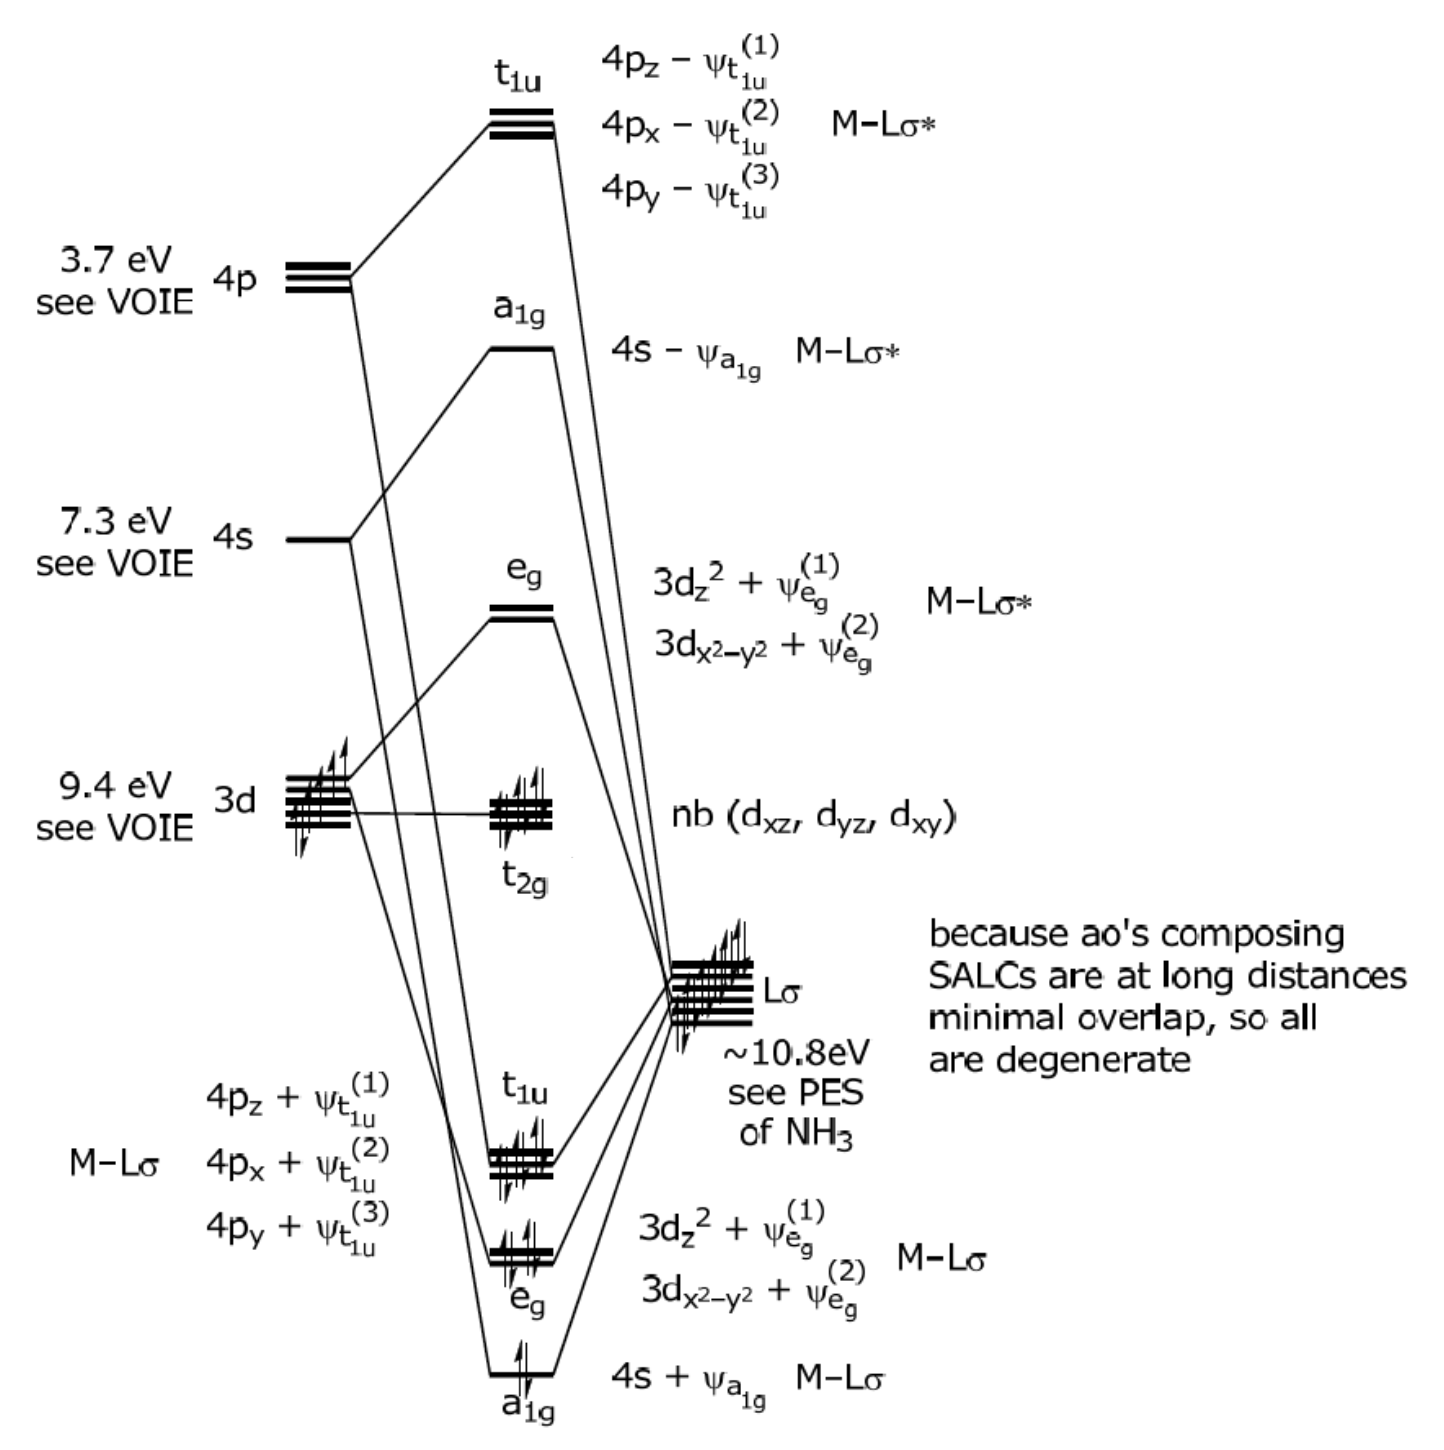
\includegraphics[width=0.6\linewidth]{../ExtFiles/MOsML6.png}
            \caption{\ce{ML6} MO diagram.}
            \label{fig:MOsML6}
        \end{figure}
        \begin{itemize}
            \item In particular, we want to be able to determine what all of the MOs on the diagram look like.
        \end{itemize}
    \end{enumerate}
    \item $\pi$-donating ligands.
    \begin{itemize}
        \item Typical $\pi$-donating ligands include halides (\ce{X}), amides (\ce{CONH2}), sulfides (\ce{S^2-}), and oxides (\ce{O^2-}).
        \item Pictures of $\sigma$- and $\pi$-donation (see Figure VI.4 of \textcite{bib:CHEM20100Notes}).
    \end{itemize}
    \item $\pi$-accepting ligands.
    \begin{itemize}
        \item Typical $\pi$-accepting ligands include \ce{CO}, \ce{NO+}, \ce{CN-}, \ce{CNR}, and \ce{PPh3}.
        \item Pictures of $\sigma$-donation and $\pi$ acceptance (see Figure VI.4 of \textcite{bib:CHEM20100Notes}).
    \end{itemize}
\end{itemize}




\end{document}